\section{Mapeamento Visual e Estatístico Completo}
\label{app:graficos_completos}

Este apêndice reúne os gráficos das trajetórias espaciais e a evolução temporal do NIS para os seis cenários testados. 
A sequência de imagens permite comparar diretamente a precisão e a consistência do EKF sintonizado com o filtro descalibrado.
Com isso, fica evidente o impacto visual da parametrização incorreta sobre as elipses de incerteza e os erros do sistema.

% ==============================================================
% PÁGINA 1: TODAS AS TRAJETÓRIAS (SINTONIZADAS E NÃO SINTONIZADAS) - SEM ALTERAÇÃO DE TAMANHO
% ==============================================================
\begin{figure*}[!htpb]
    \centering
    
    % --- PARTE A: SINTONIZADAS ---
    % Linha 1
    \begin{minipage}[b]{0.24\linewidth}
        \centering
        
\includegraphics[width=\linewidth]{Figuras/C1/sintonizado/simulacao_círculo_1_traj.png}
        \vspace{1mm} \par {\small (a) Círculo}
    \end{minipage}
    \hfill
    \begin{minipage}[b]{0.24\linewidth}
        \centering
        
\includegraphics[width=\linewidth]{Figuras/C2/sintonizado/simulacao_quadrado_1_traj.png}
        \vspace{1mm} \par {\small (b) Quadrado}
    \end{minipage}
    \hfill
    \begin{minipage}[b]{0.24\linewidth}
        \centering
        
\includegraphics[width=\linewidth]{Figuras/C3/sintonizado/simulacao_tangente_hiperbólica_1_traj.png}
        \vspace{1mm} \par {\small (c) Tangente Hiperbólica}
    \end{minipage}
    
    \vspace{3mm} % Espaço entre as linhas
    
    % Linha 2
    \begin{minipage}[b]{0.24\linewidth}
        \centering
        
\includegraphics[width=\linewidth]{Figuras/C4/sintonizado/simulacao_lemniscata_1_traj.png}
        \vspace{1mm} \par {\small (d) Lemniscata}
    \end{minipage}
    \hfill
    \begin{minipage}[b]{0.24\linewidth}
        \centering
        
\includegraphics[width=\linewidth]{Figuras/C5/sintonizado/simulacao_aleatória_1_traj.png}
        \vspace{1mm} \par {\small (e) Aleatória}
    \end{minipage}
    \hfill
    \begin{minipage}[b]{0.24\linewidth}
        \centering
        
\includegraphics[width=\linewidth]{Figuras/C6/sintonizado/simulacao_oclusão_1_traj.png}
        \vspace{1mm} \par {\small (f) Oclusão}
    \end{minipage}
    
    \caption{Trajetórias estimadas na \textbf{condição sintonizada}. Observa-se o rastreamento preciso da dinâmica do alvo e a mitigação contínua do ruído de observação, evidenciando o desempenho ideal do filtro.}
    \label{fig:app_traj_sintonizadas_grid}

    \vspace{8mm} % ESPAÇO ENTRE OS DOIS BLOCOS DE TRAJETÓRIA

    % --- PARTE B: NÃO SINTONIZADAS ---
    % Linha 1
    \begin{minipage}[b]{0.24\linewidth}
        \centering
        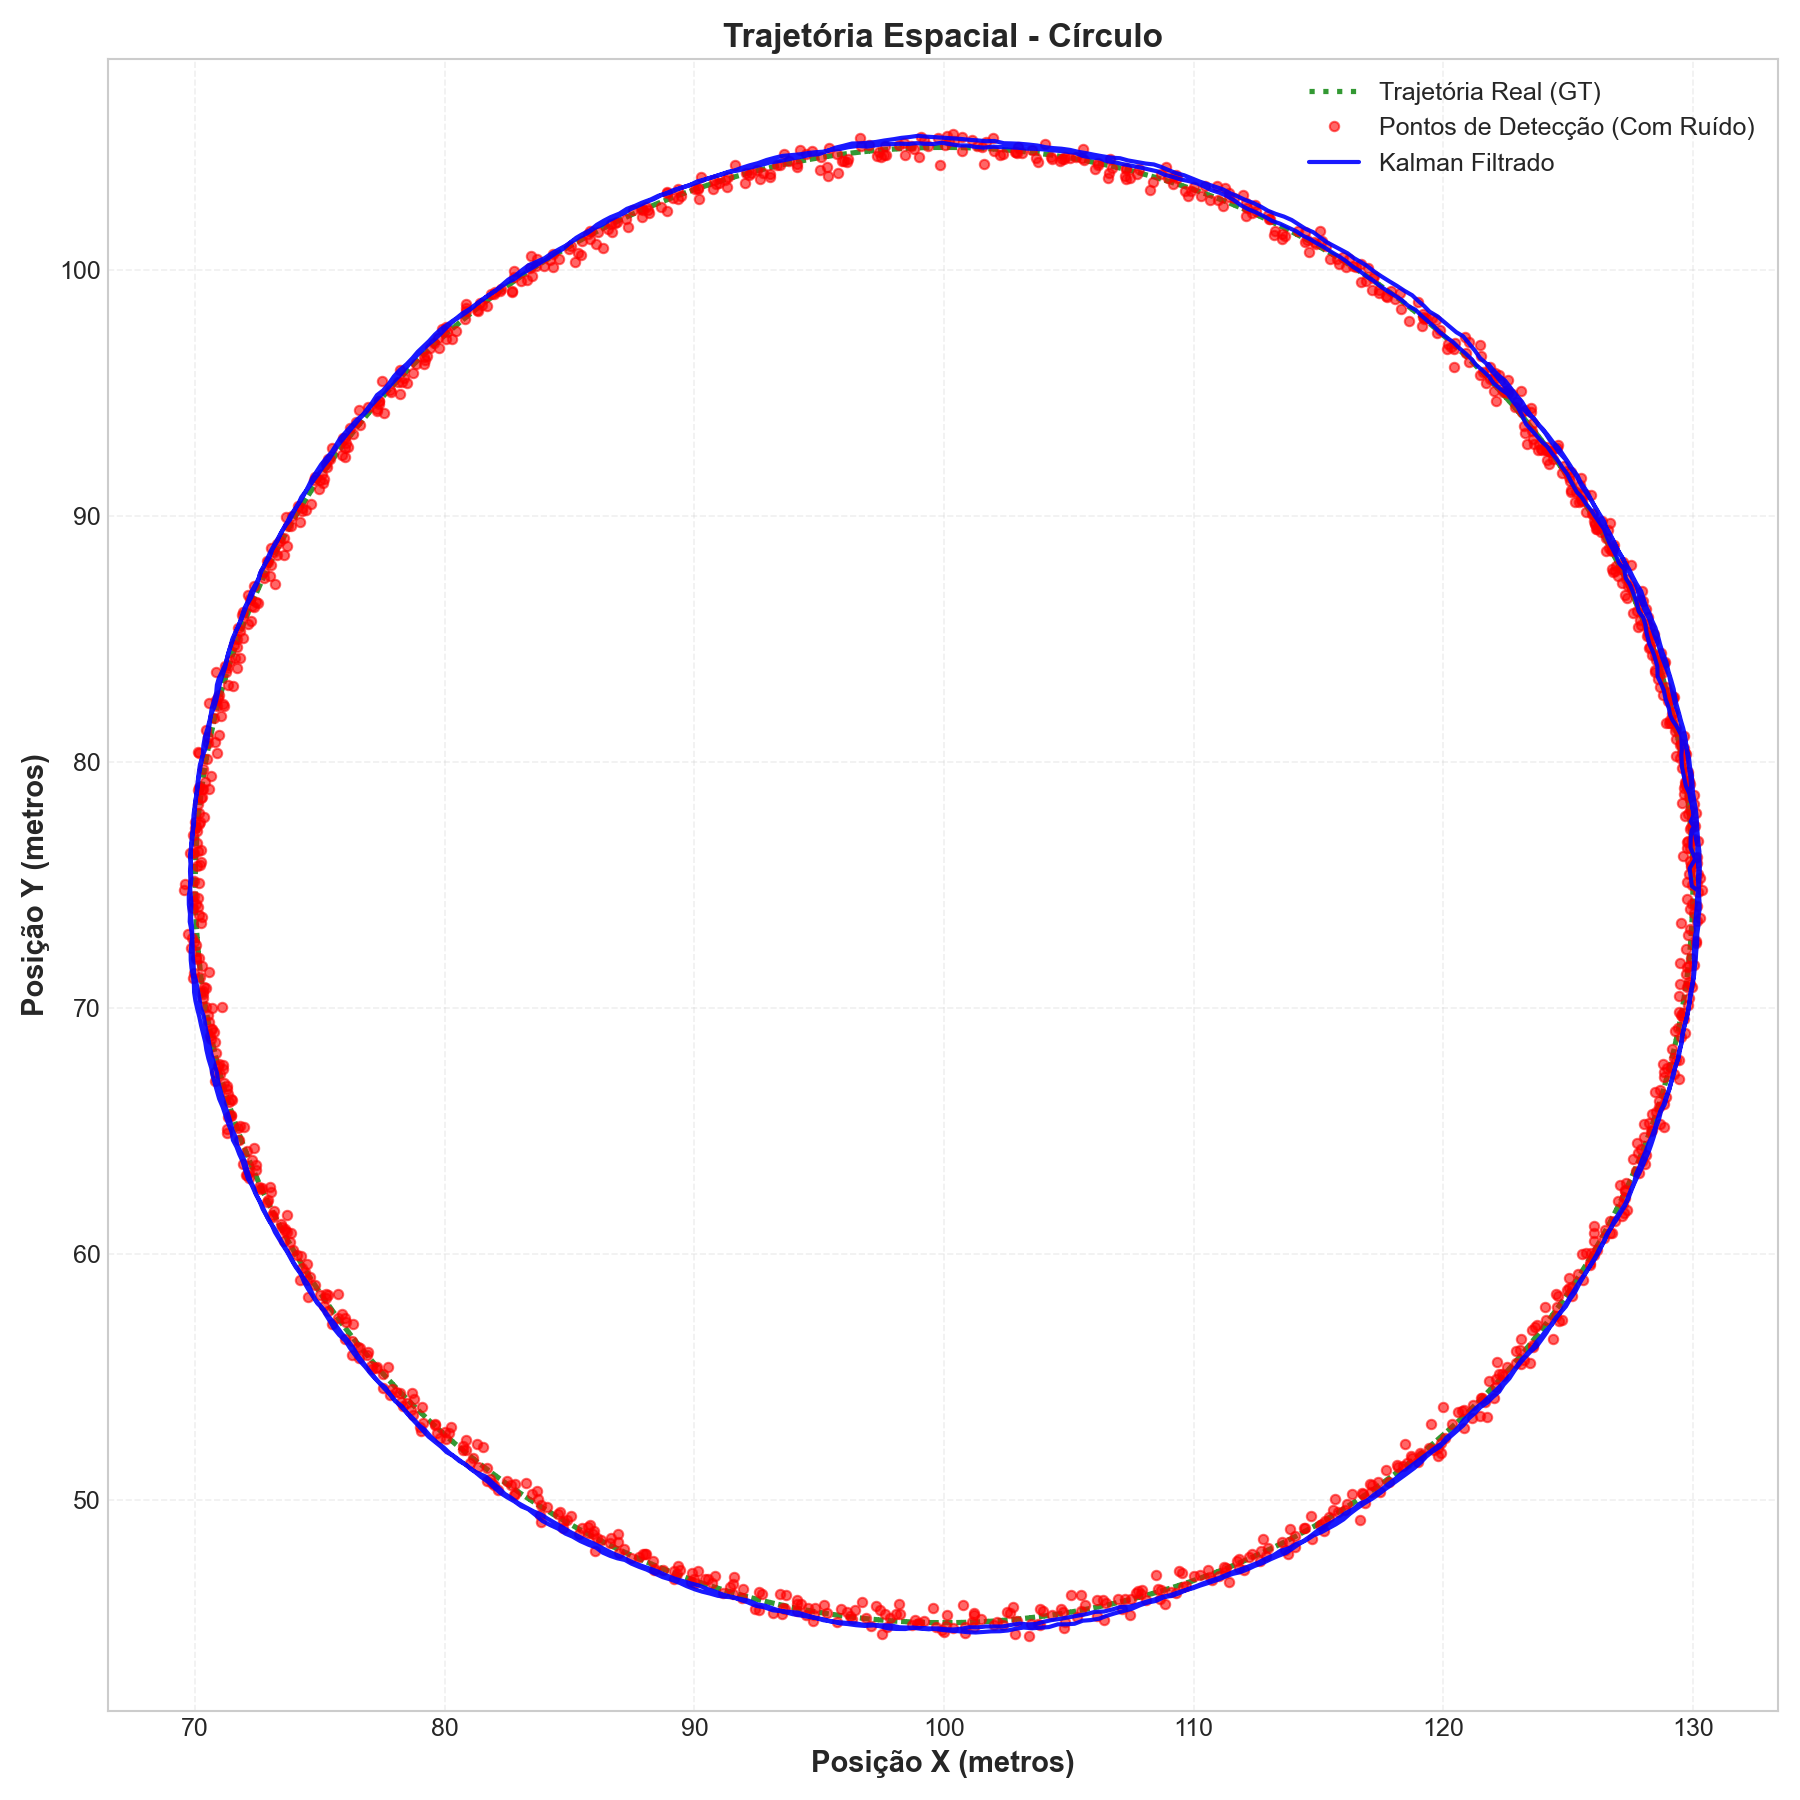
\includegraphics[width=\linewidth]{Figuras/C1/nsintonizado/simulacao_círculo_1_traj.png}
        \vspace{1mm} \par {\small (a) Círculo}
    \end{minipage}
    \hfill
    \begin{minipage}[b]{0.24\linewidth}
        \centering
        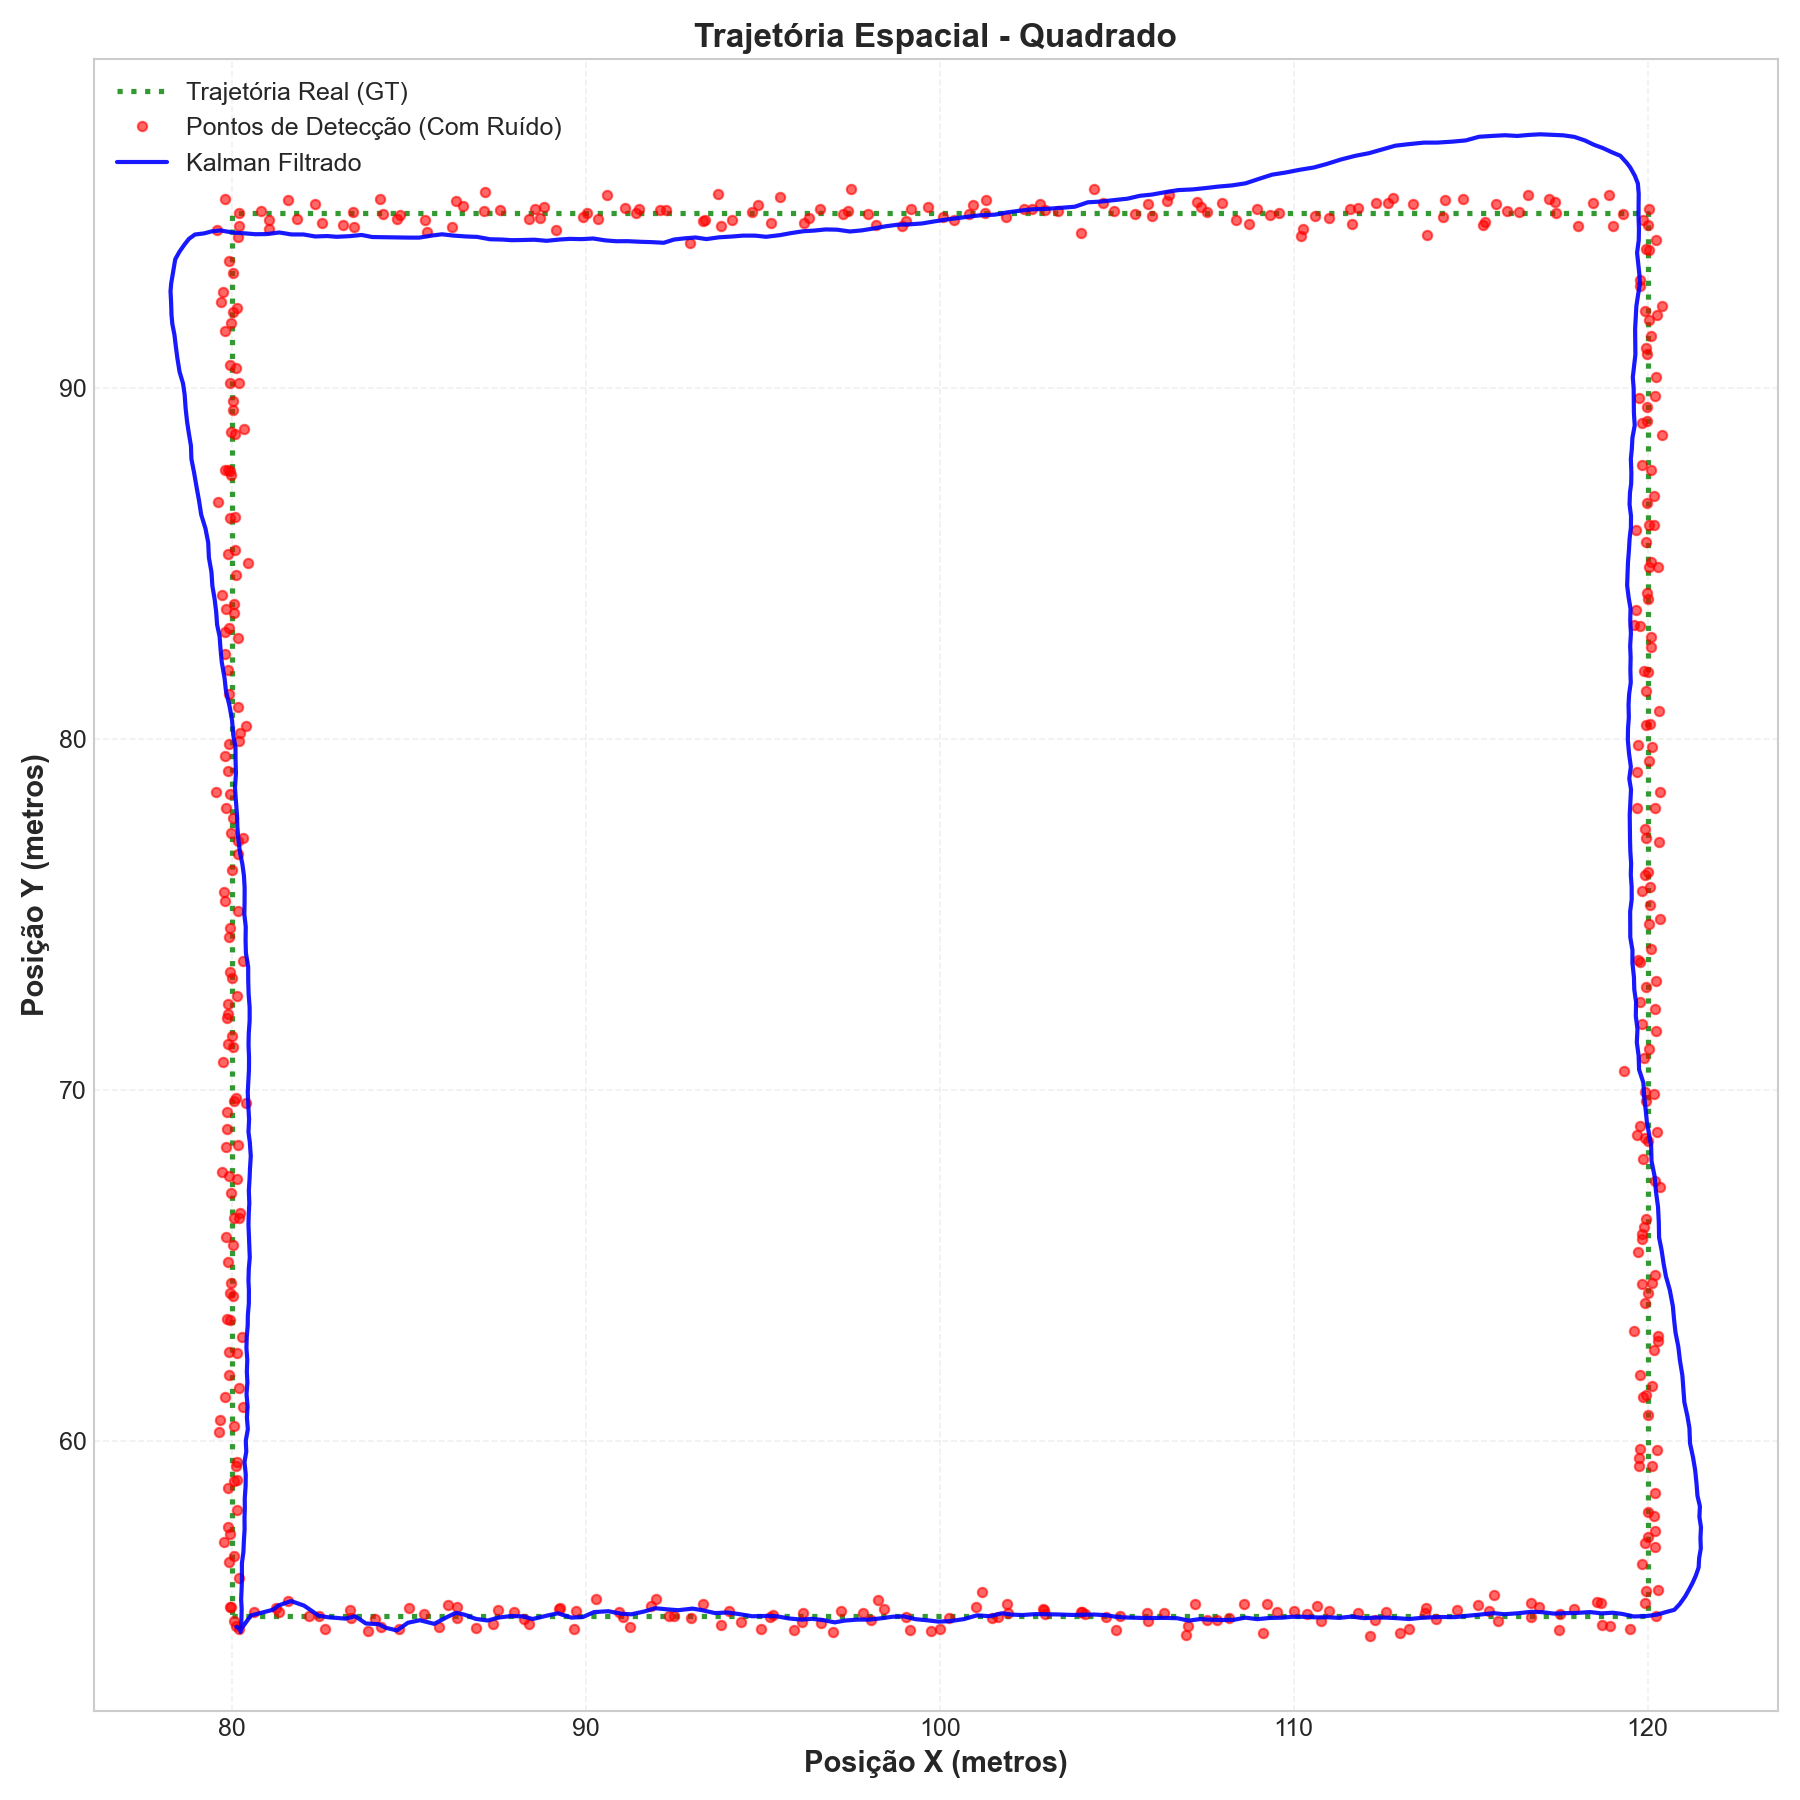
\includegraphics[width=\linewidth]{Figuras/C2/nsintonizado/simulacao_quadrado_1_traj.png}
        \vspace{1mm} \par {\small (b) Quadrado}
    \end{minipage}
    \hfill
    \begin{minipage}[b]{0.24\linewidth}
        \centering
        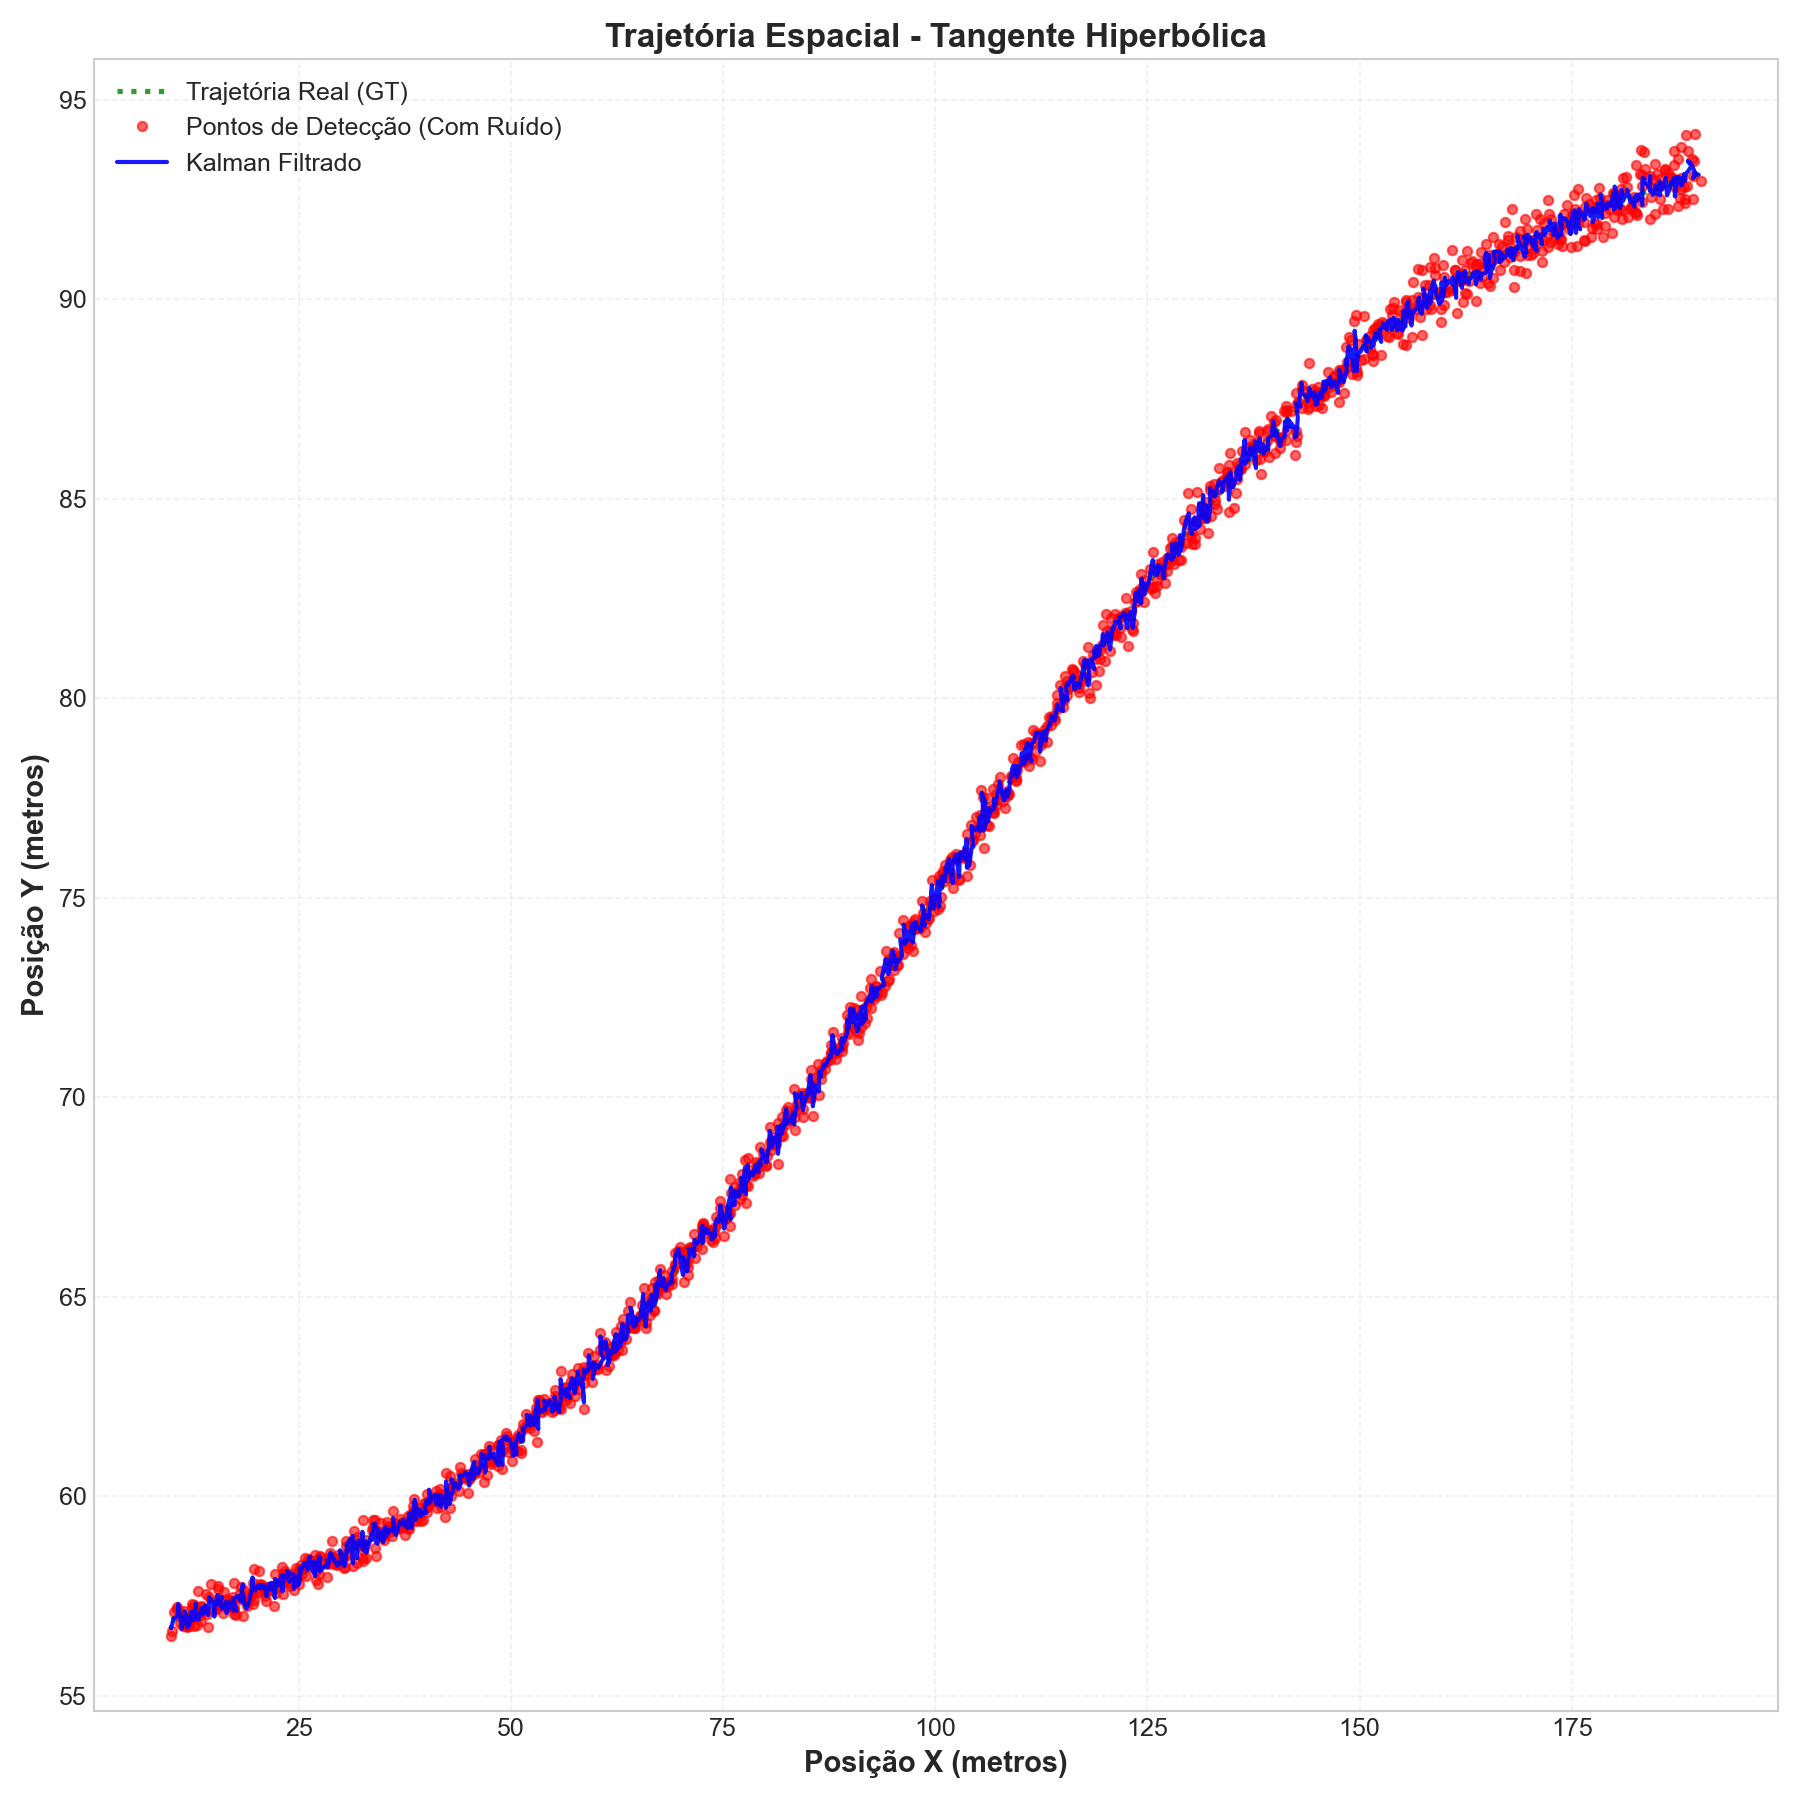
\includegraphics[width=\linewidth]{Figuras/C3/nsintonizado/simulacao_tangente_hiperbólica_1_traj.png}
        \vspace{1mm} \par {\small (c) Tangente Hiperbólica}
    \end{minipage}
    
    \vspace{3mm}
    
    % Linha 2
    \begin{minipage}[b]{0.24\linewidth}
        \centering
        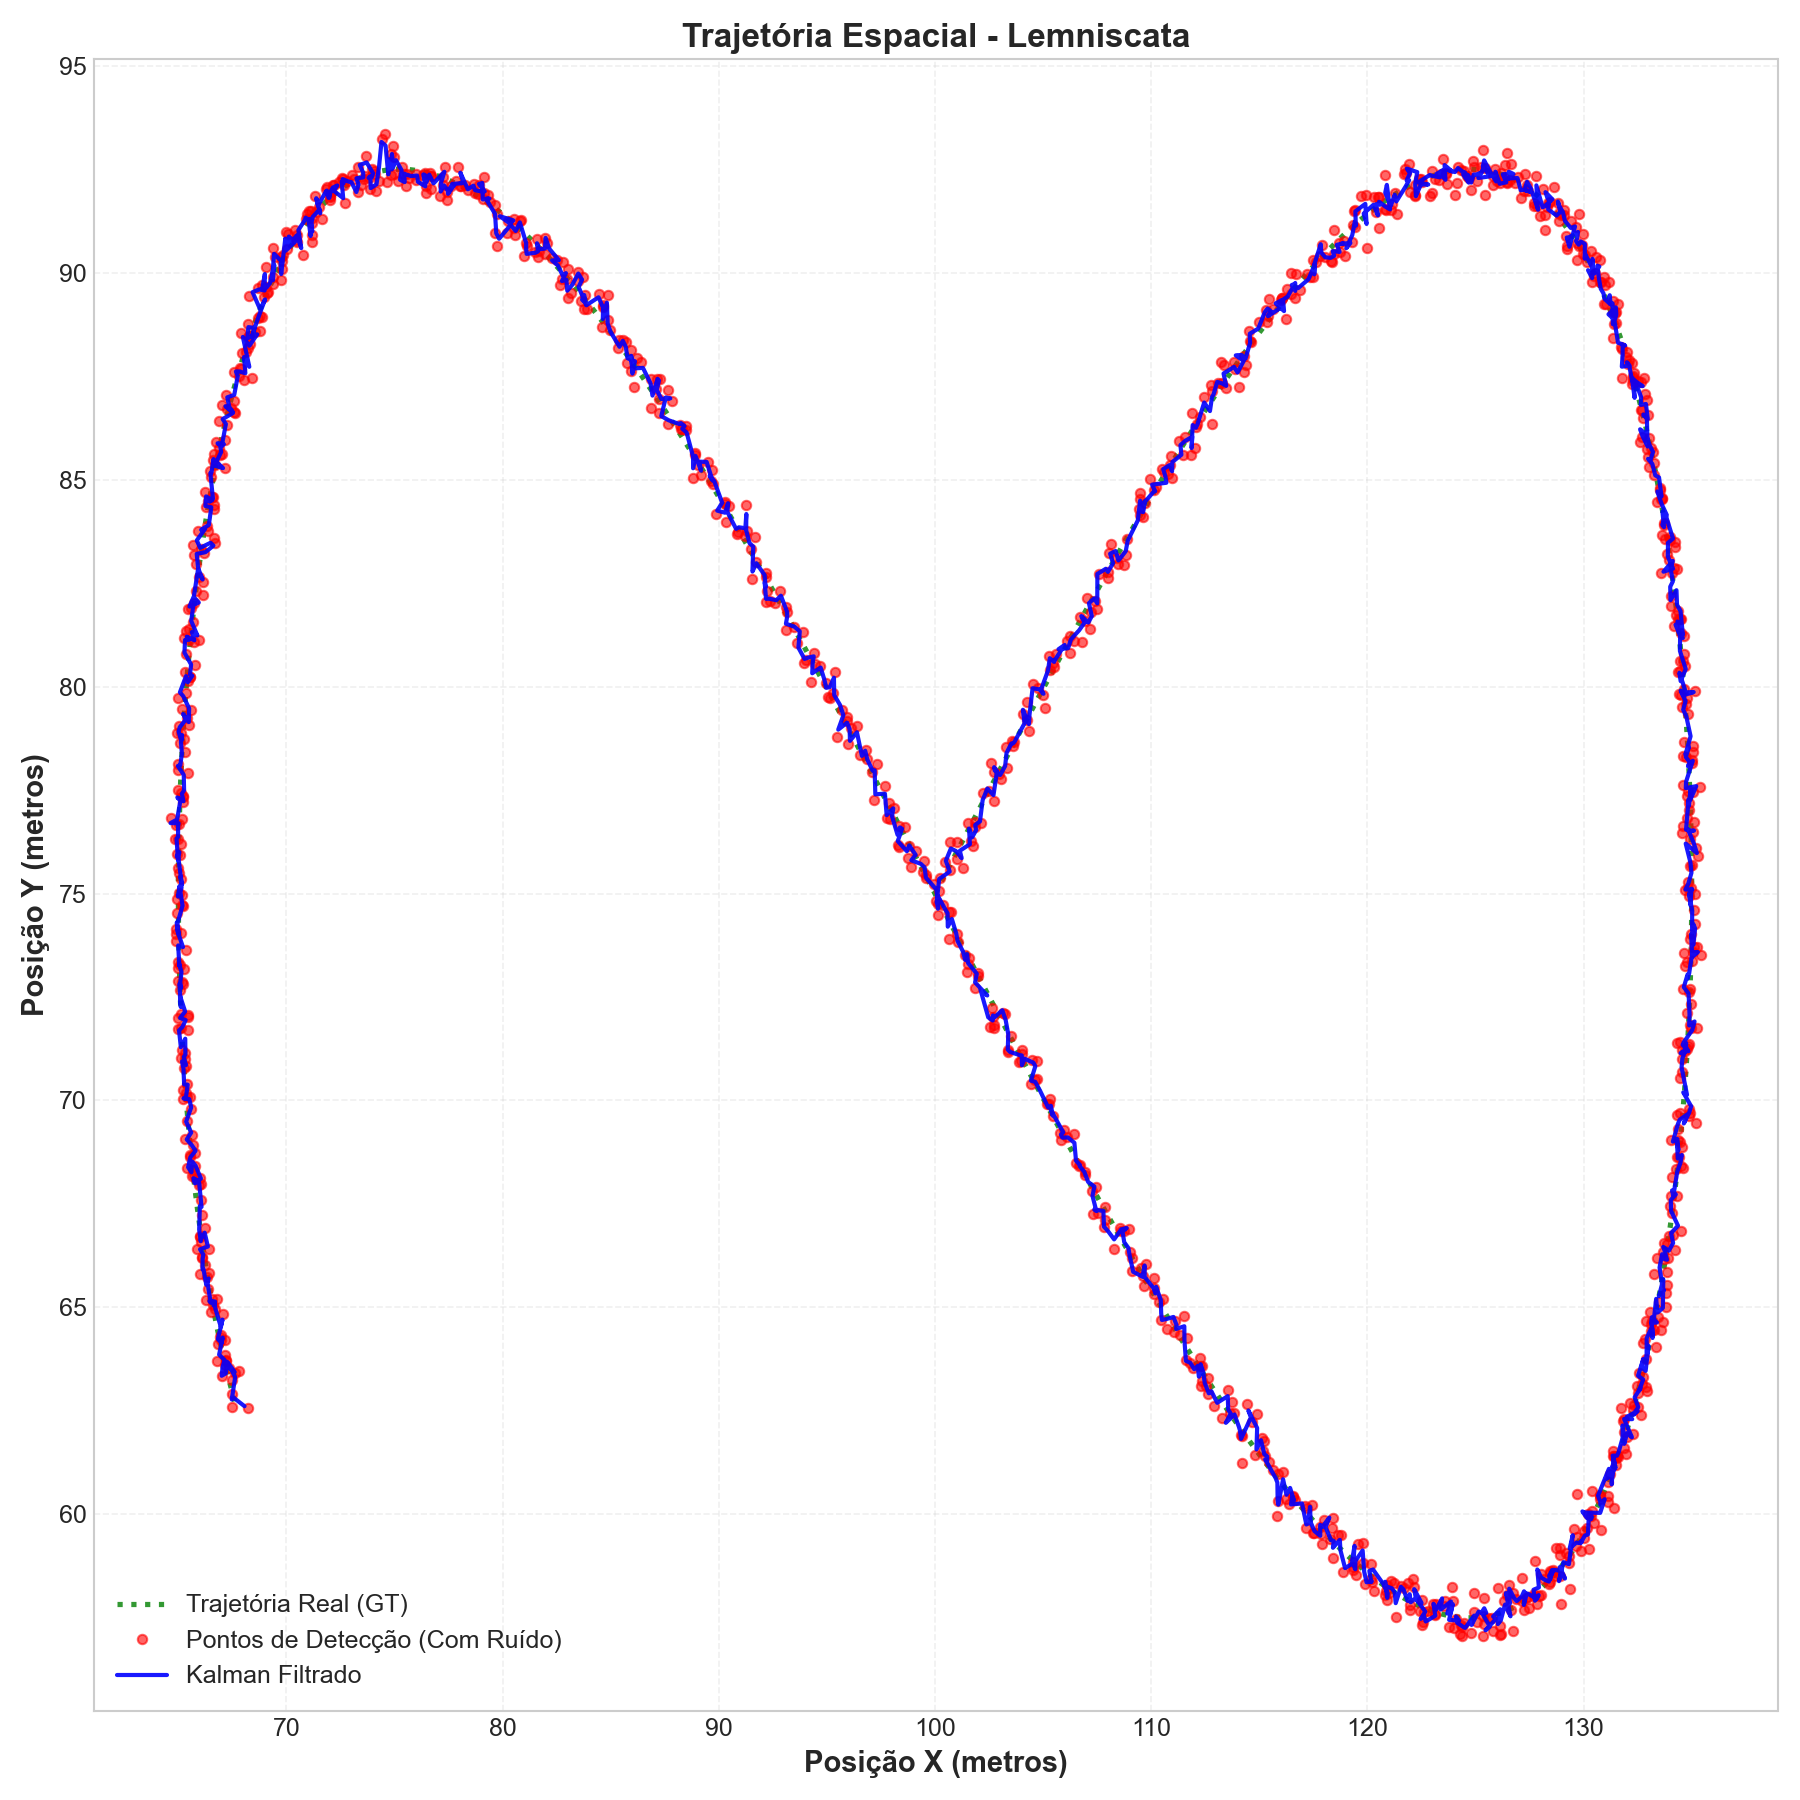
\includegraphics[width=\linewidth]{Figuras/C4/nsintonizado/simulacao_lemniscata_1_traj.png}
        \vspace{1mm} \par {\small (d) Lemniscata}
    \end{minipage}
    \hfill
    \begin{minipage}[b]{0.24\linewidth}
        \centering
        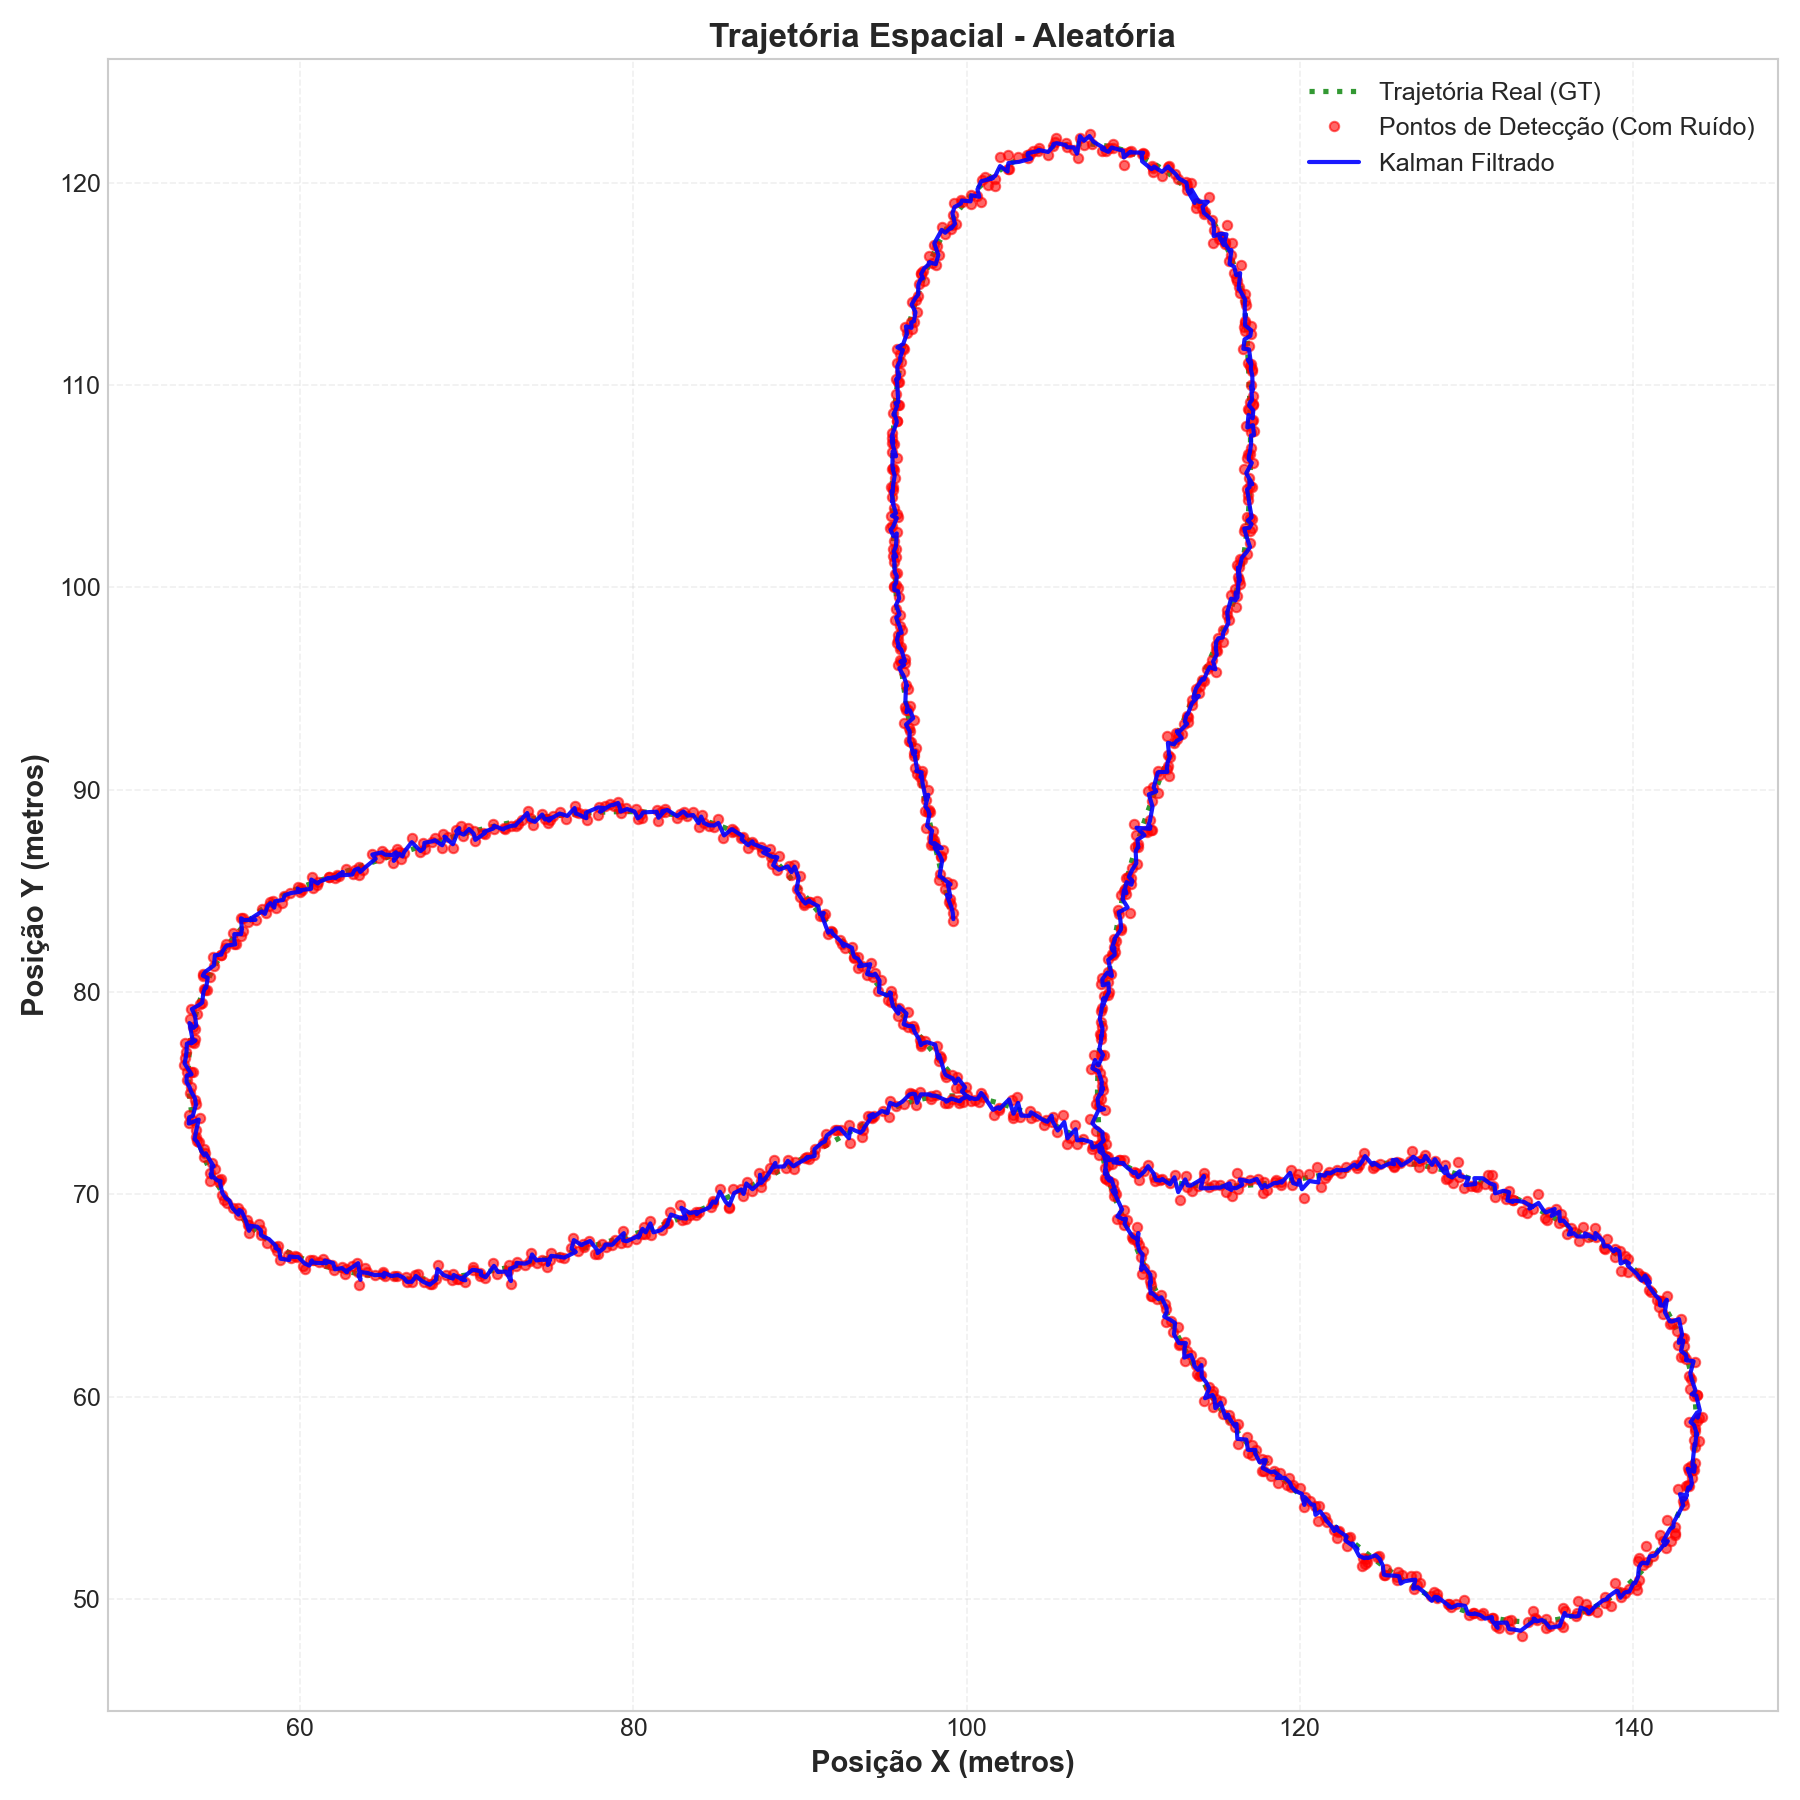
\includegraphics[width=\linewidth]{Figuras/C5/nsintonizado/simulacao_aleatória_1_traj.png}
        \vspace{1mm} \par {\small (e) Aleatória}
    \end{minipage}
    \hfill
    \begin{minipage}[b]{0.24\linewidth}
        \centering
        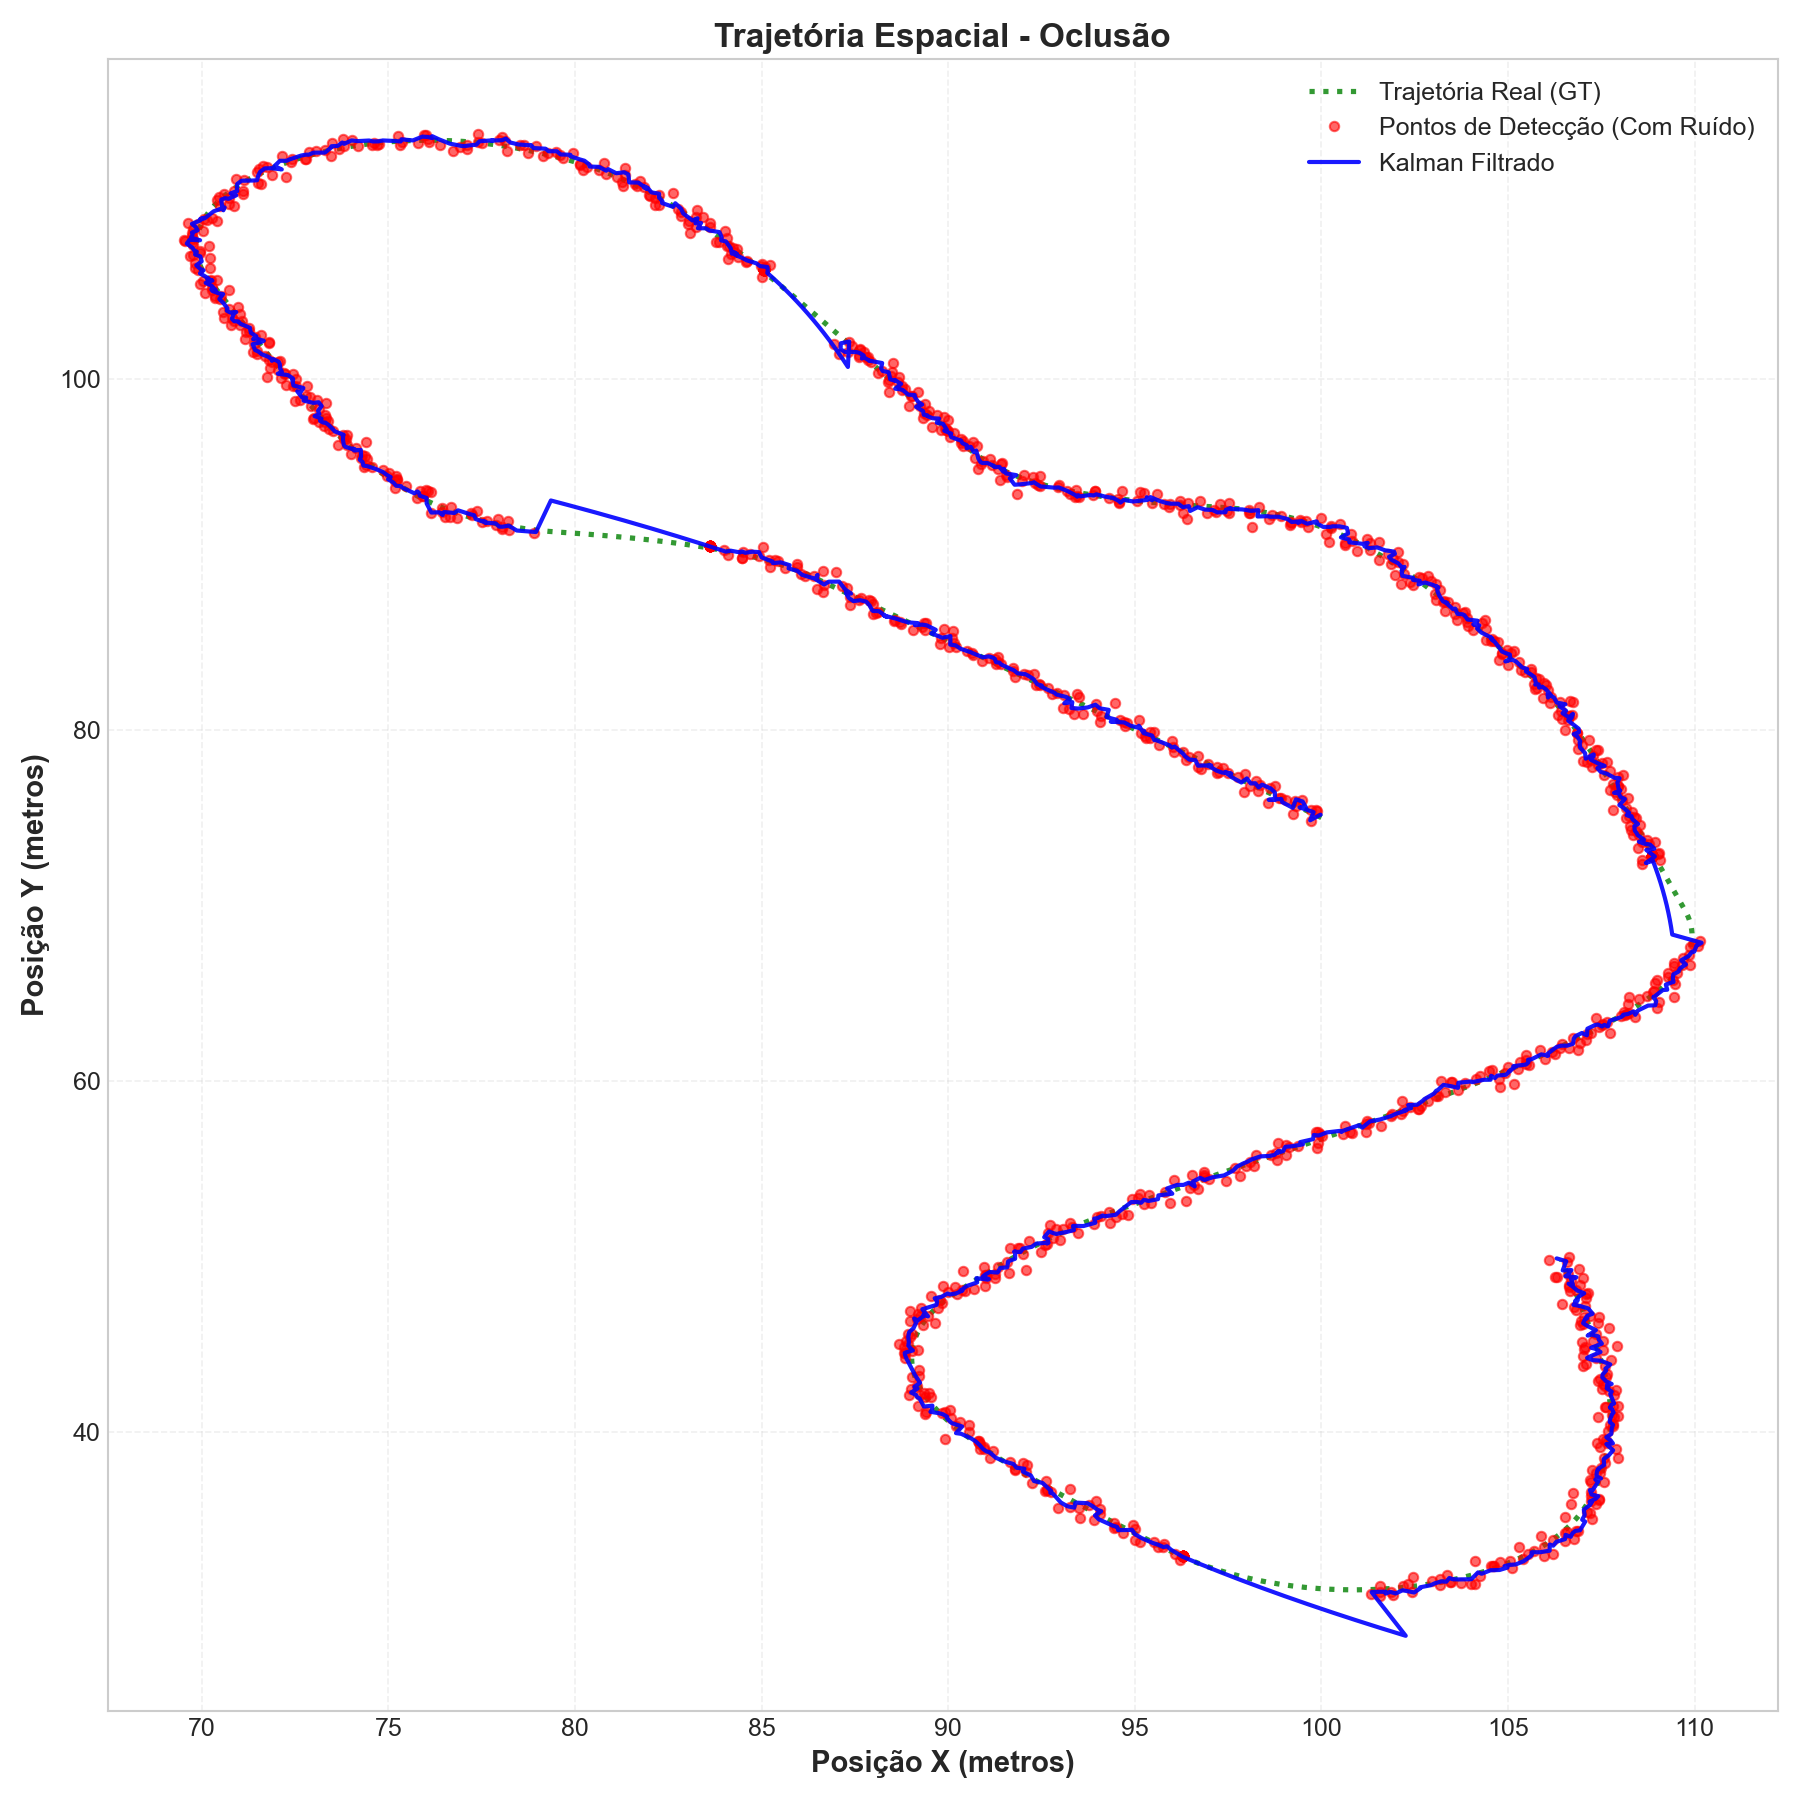
\includegraphics[width=\linewidth]{Figuras/C6/nsintonizado/simulacao_oclusão_1_traj.png}
        \vspace{1mm} \par {\small (f) Oclusão}
    \end{minipage}
    
    \caption{Trajetórias estimadas na \textbf{condição não sintonizada}. Notam-se divergências significativas em relação à verdade terrestre (\textit{ground truth}), com evidentes atrasos de fase e sobreposições bruscas nas curvas.}
    \label{fig:app_traj_naosintonizadas_grid}
\end{figure*}

% QUEBRA DE PÁGINA OBRIGATÓRIA
\clearpage


% ==============================================================
% PÁGINA 2: TODOS OS GRÁFICOS RMSE (SINTONIZADOS E NÃO SINTONIZADOS) - MAIORES
% ==============================================================
\begin{figure*}[!htpb]
    \centering
    
    % --- PARTE A: NIS SINTONIZADO ---
    % Linha 1
    \begin{minipage}[b]{0.32\linewidth}
        \centering
        
\includegraphics[width=\linewidth]{Figuras/C1/sintonizado/simulacao_círculo_2_rms.png}
        \vspace{1mm} \par {\small (a) Círculo}
    \end{minipage}
    \hfill
    \begin{minipage}[b]{0.32\linewidth}
        \centering
        
\includegraphics[width=\linewidth]{Figuras/C2/sintonizado/simulacao_quadrado_2_rms.png}
        \vspace{1mm} \par {\small (b) Quadrado}
    \end{minipage}
    \hfill
    \begin{minipage}[b]{0.32\linewidth}
        \centering
        
\includegraphics[width=\linewidth]{Figuras/C3/sintonizado/simulacao_tangente_hiperbólica_2_rms.png}
        \vspace{1mm} \par {\small (c) Tangente Hiperbólica}
    \end{minipage}
    
    \vspace{3mm}
    
    % Linha 2
    \begin{minipage}[b]{0.32\linewidth}
        \centering
        
\includegraphics[width=\linewidth]{Figuras/C4/sintonizado/simulacao_lemniscata_2_rms.png}
        \vspace{1mm} \par {\small (d) Lemniscata}
    \end{minipage}
    \hfill
    \begin{minipage}[b]{0.32\linewidth}
        \centering
        
\includegraphics[width=\linewidth]{Figuras/C5/sintonizado/simulacao_aleatória_2_rms.png}
        \vspace{1mm} \par {\small (e) Aleatória}
    \end{minipage}
    \hfill
    \begin{minipage}[b]{0.32\linewidth}
        \centering
        
\includegraphics[width=\linewidth]{Figuras/C6/sintonizado/simulacao_oclusão_2_rms.png}
        \vspace{1mm} \par {\small (f) Oclusão}
    \end{minipage}
    
    \caption{Evolução temporal da métrica RMSE para a \textbf{condição sintonizada}}
    \label{fig:app_rmse_sintonizado_grid}

    \vspace{8mm} % ESPAÇO ENTRE OS DOIS BLOCOS DE NIS

    % --- PARTE B: NIS NÃO SINTONIZADO ---
    % Linha 1
    \begin{minipage}[b]{0.32\linewidth}
        \centering
        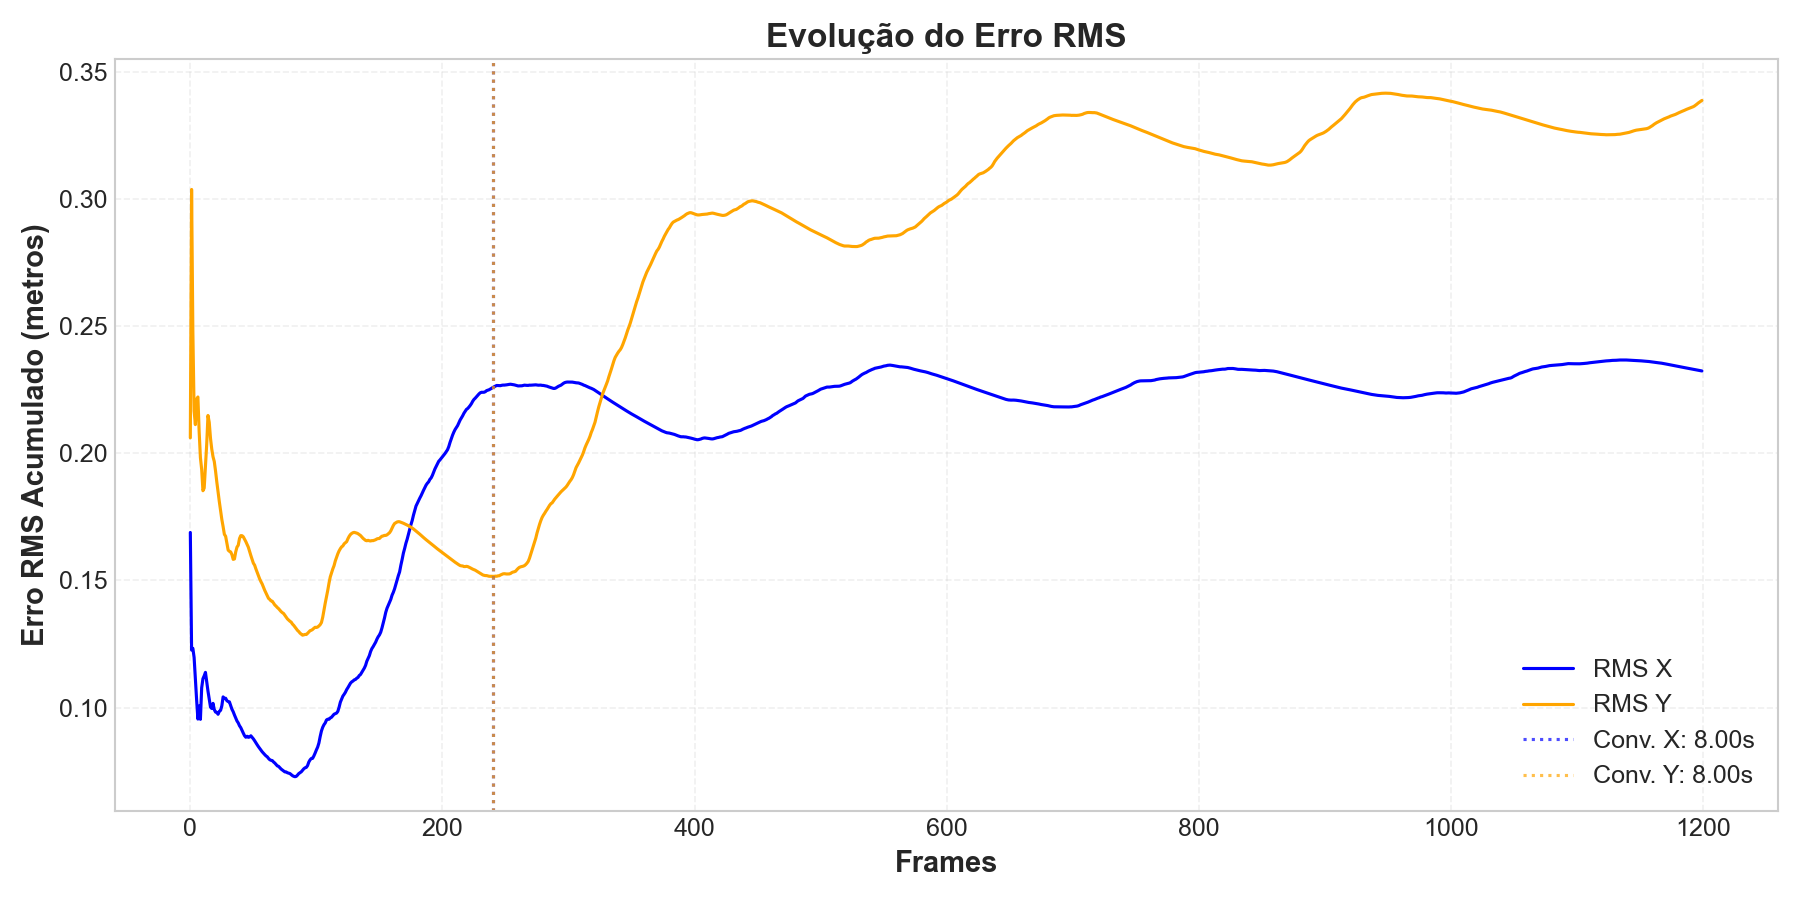
\includegraphics[width=\linewidth]{Figuras/C1/nsintonizado/simulacao_círculo_2_rms.png}
        \vspace{1mm} \par {\small (a) Círculo}
    \end{minipage}
    \hfill
    \begin{minipage}[b]{0.32\linewidth}
        \centering
        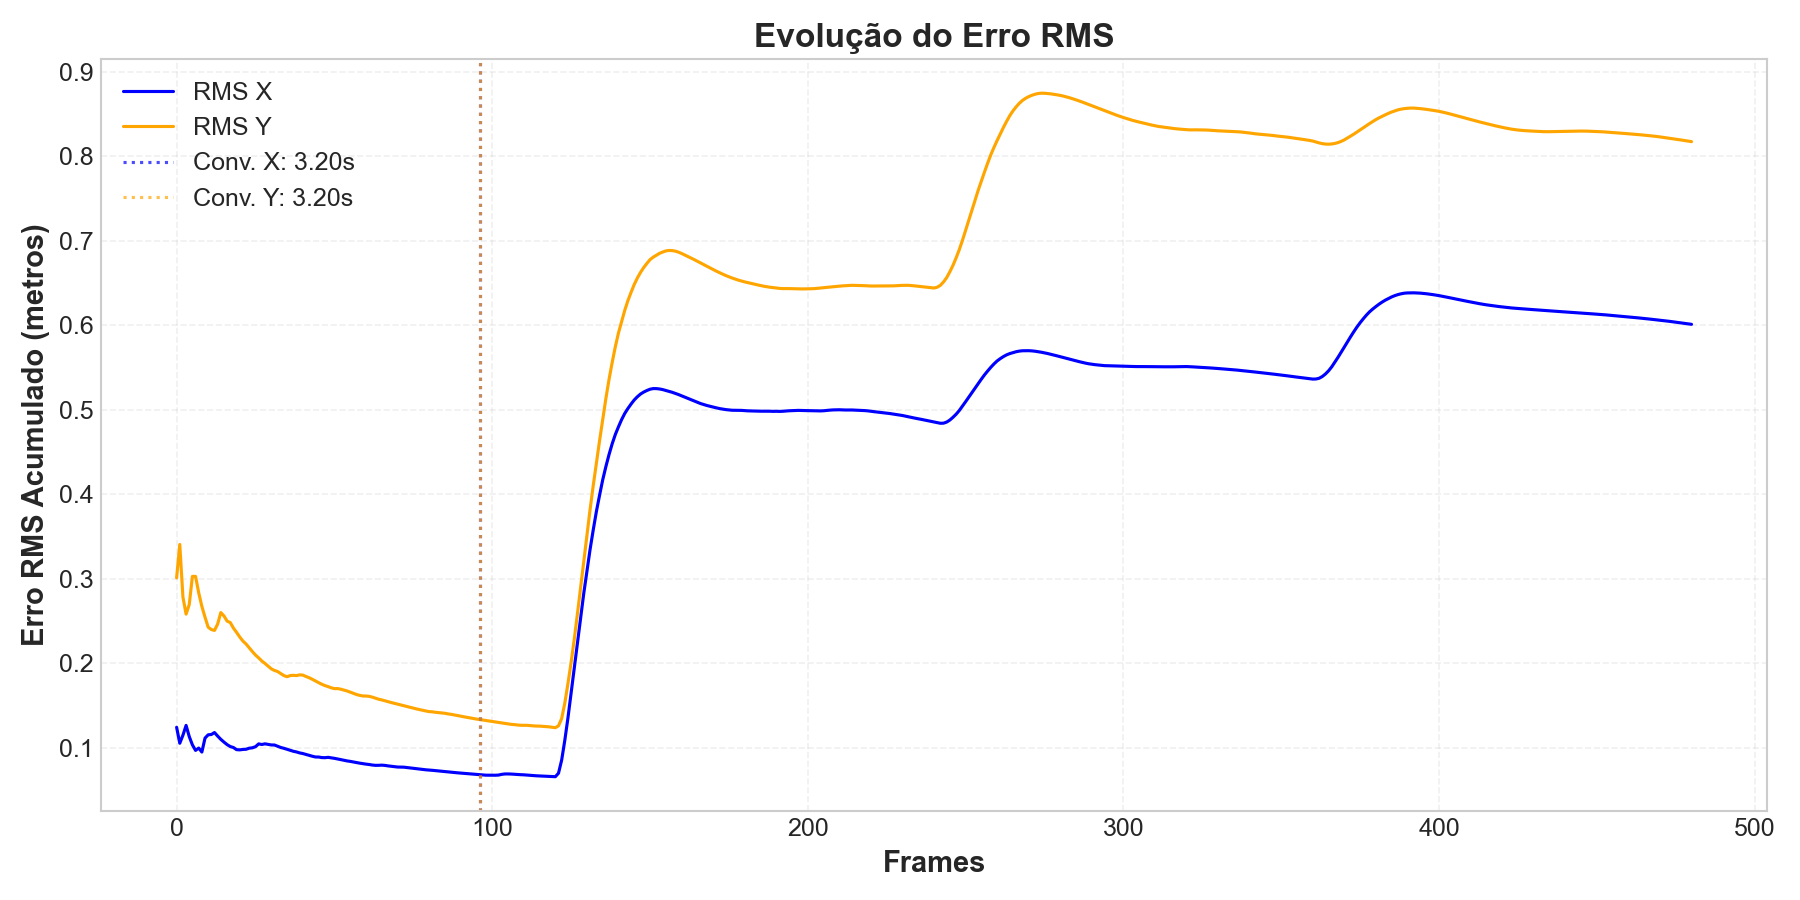
\includegraphics[width=\linewidth]{Figuras/C2/nsintonizado/simulacao_quadrado_2_rms.png}
        \vspace{1mm} \par {\small (b) Quadrado}
    \end{minipage}
    \hfill
    \begin{minipage}[b]{0.32\linewidth}
        \centering
        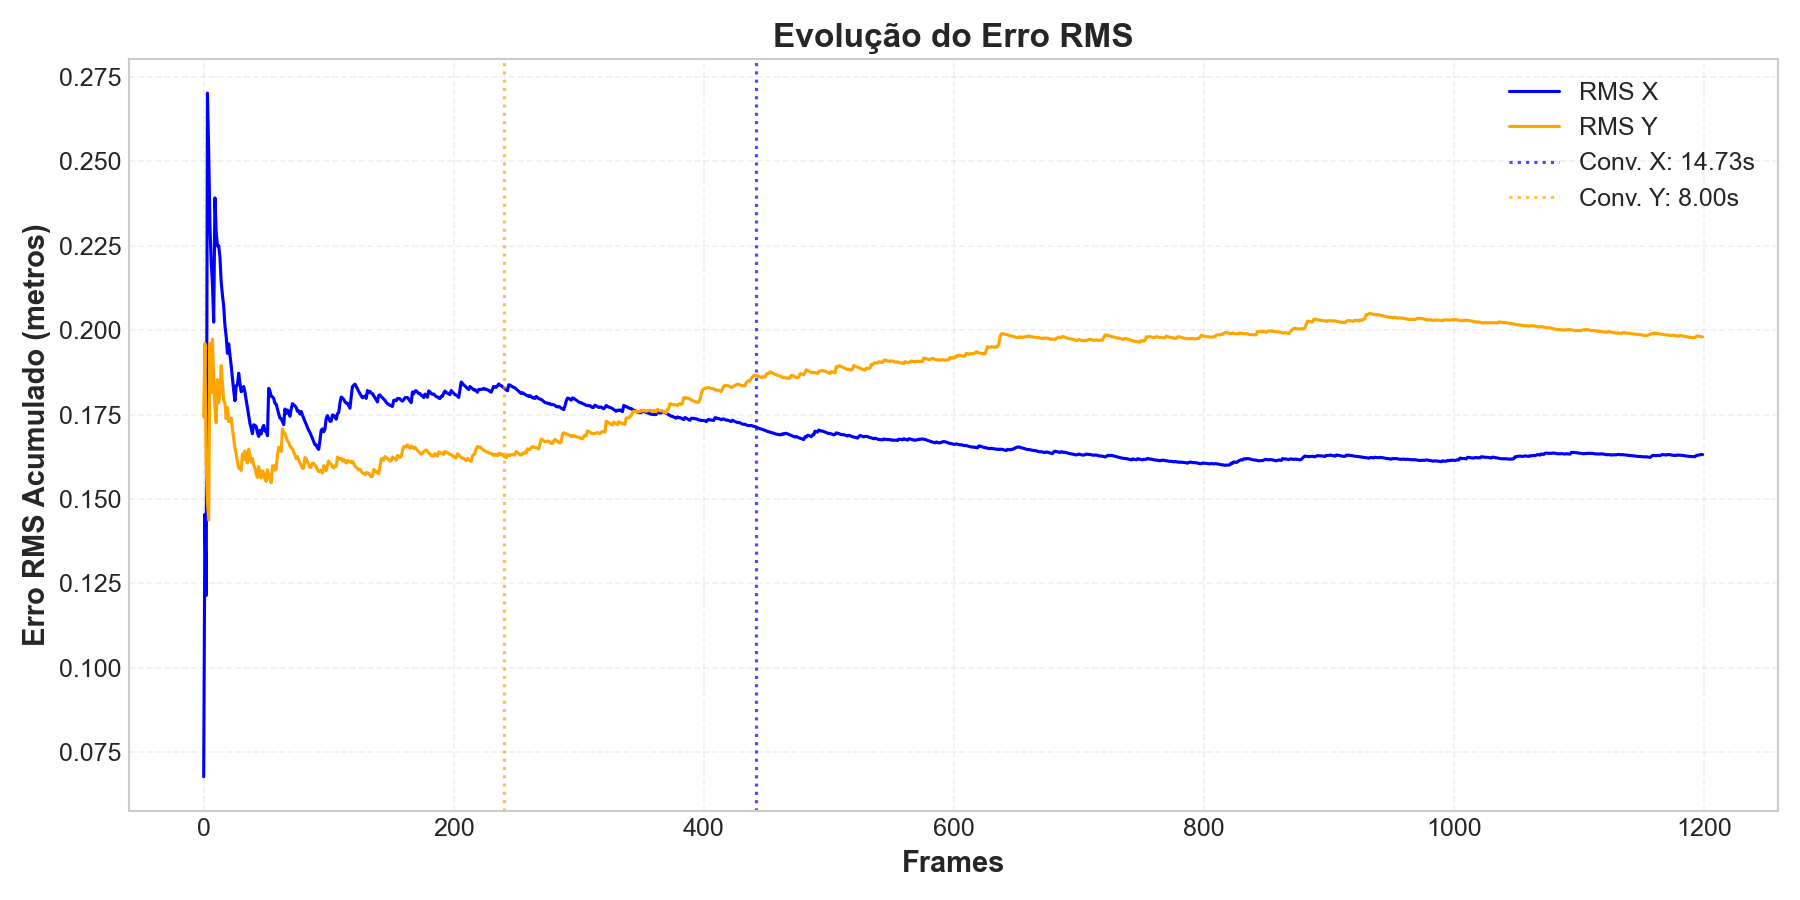
\includegraphics[width=\linewidth]{Figuras/C3/nsintonizado/simulacao_tangente_hiperbólica_2_rms.png}
        \vspace{1mm} \par {\small (c) Tangente Hiperbólica}
    \end{minipage}
    
    \vspace{3mm}
    
    % Linha 2
    \begin{minipage}[b]{0.32\linewidth}
        \centering
        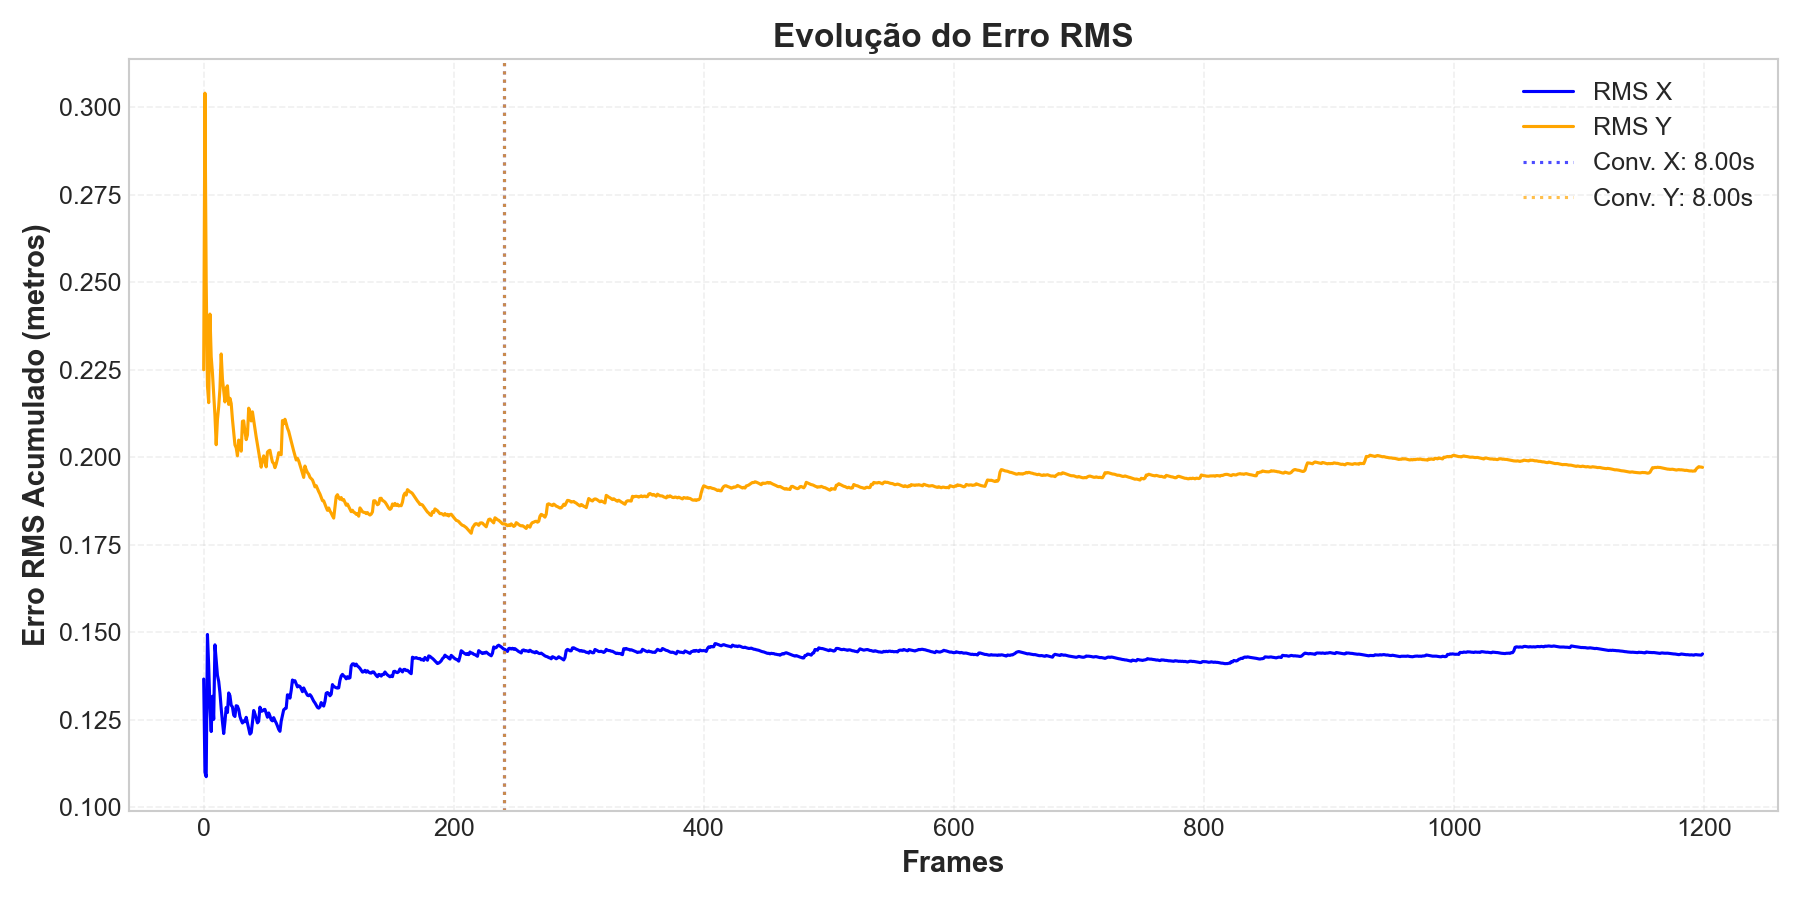
\includegraphics[width=\linewidth]{Figuras/C4/nsintonizado/simulacao_lemniscata_2_rms.png}
        \vspace{1mm} \par {\small (d) Lemniscata}
    \end{minipage}
    \hfill
    \begin{minipage}[b]{0.32\linewidth}
        \centering
        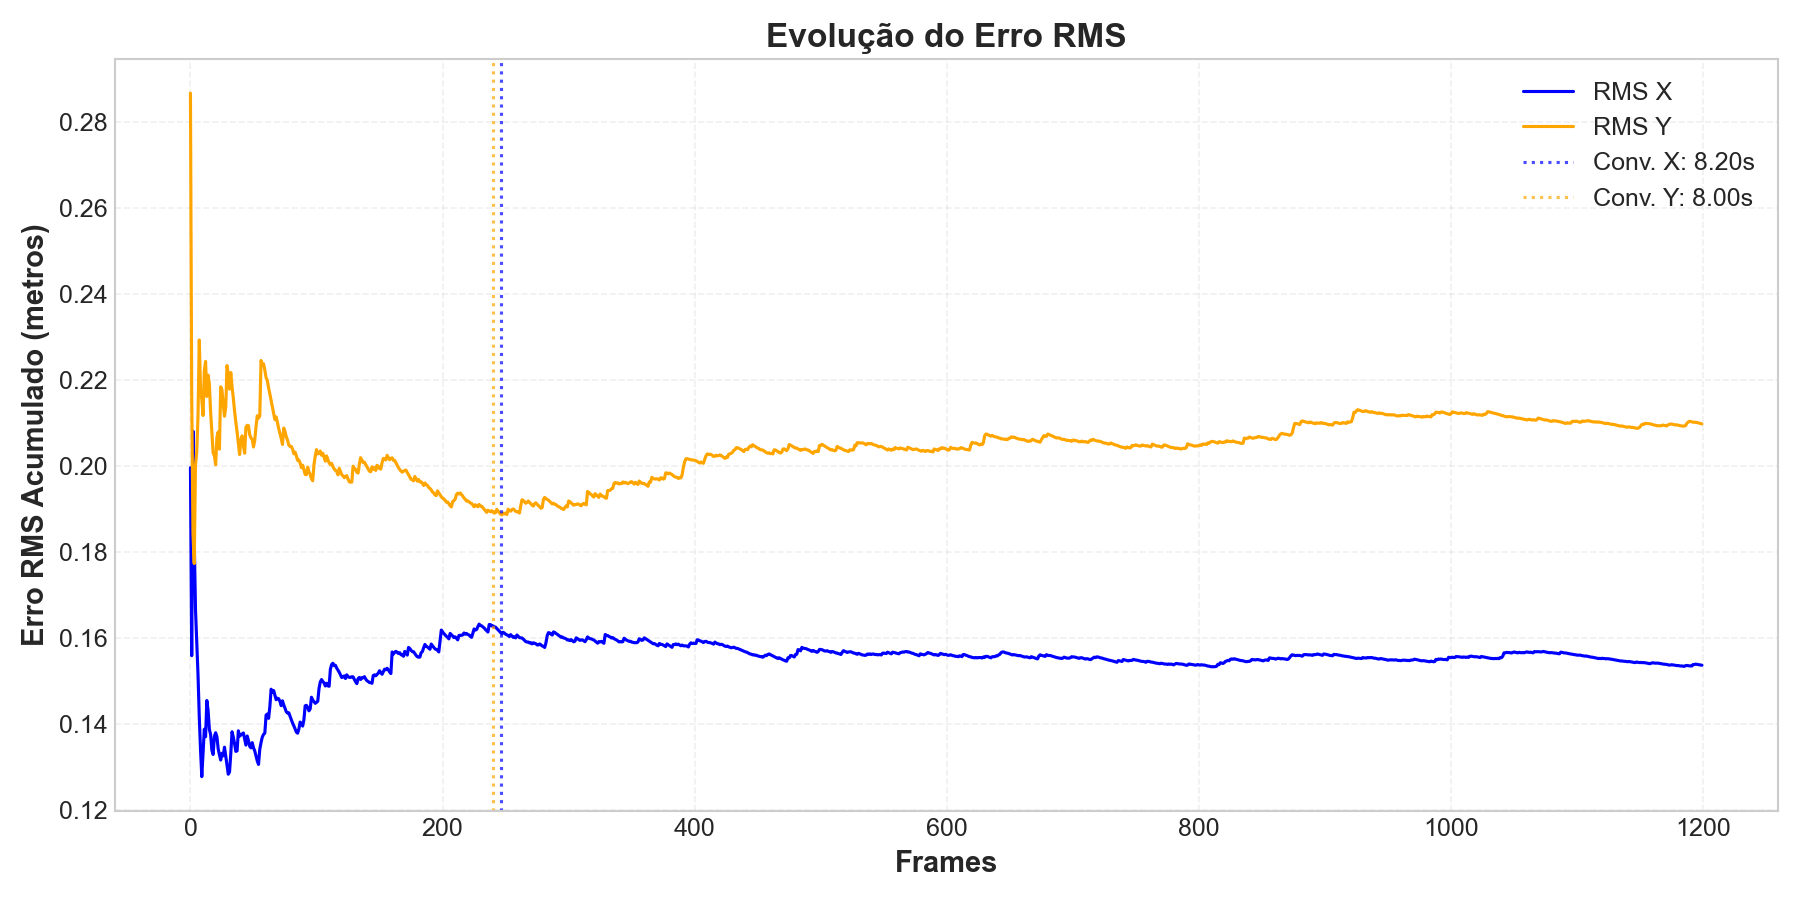
\includegraphics[width=\linewidth]{Figuras/C5/nsintonizado/simulacao_aleatória_2_rms.png}
        \vspace{1mm} \par {\small (e) Aleatória}
    \end{minipage}
    \hfill
    \begin{minipage}[b]{0.32\linewidth}
        \centering
        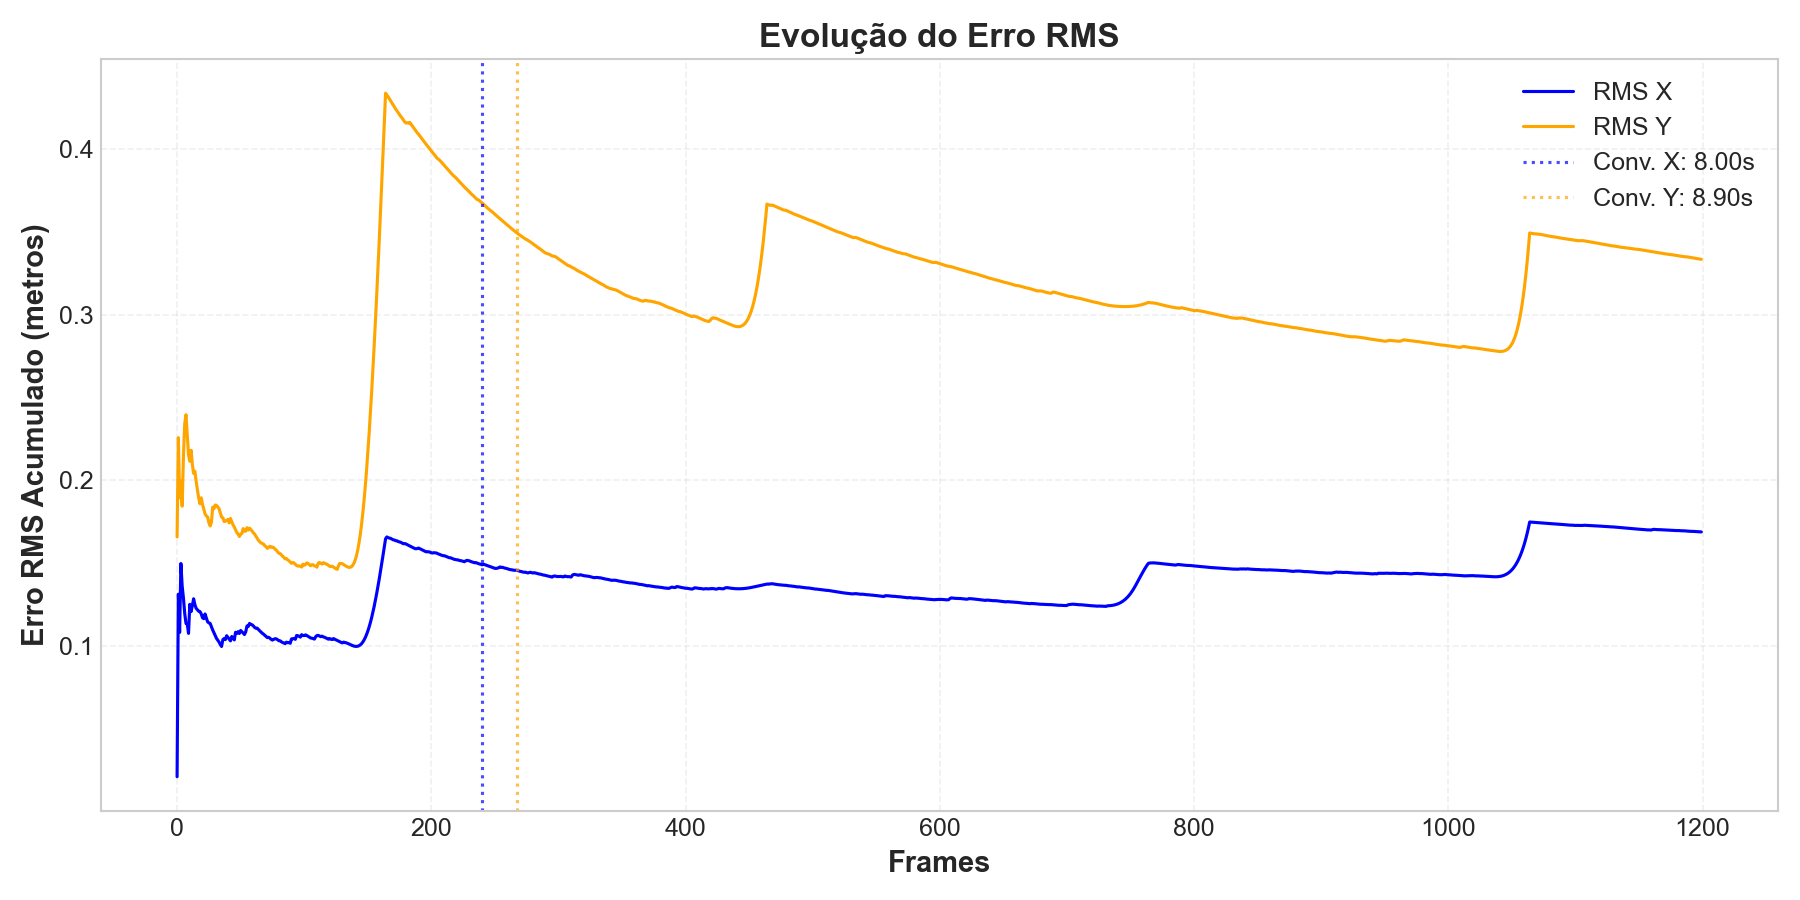
\includegraphics[width=\linewidth]{Figuras/C6/nsintonizado/simulacao_oclusão_2_rms.png}
        \vspace{1mm} \par {\small (f) Oclusão}
    \end{minipage}
    
    \caption{Evolução temporal da métrica RMSE para a \textbf{condição não sintonizada}.}
    \label{fig:app_rmse_naosintonizado_grid}
\end{figure*}

% QUEBRA DE PÁGINA OBRIGATÓRIA
\clearpage

% ==============================================================
% PÁGINA 3: TODOS OS GRÁFICOS NIS (SINTONIZADOS E NÃO SINTONIZADOS) - MAIORES
% ==============================================================
\begin{figure*}[!htpb]
    \centering
    
    % --- PARTE A: NIS SINTONIZADO ---
    % Linha 1
    \begin{minipage}[b]{0.32\linewidth}
        \centering
        
\includegraphics[width=\linewidth]{Figuras/C1/sintonizado/simulacao_círculo_4_nis.png}
        \vspace{1mm} \par {\small (a) Círculo}
    \end{minipage}
    \hfill
    \begin{minipage}[b]{0.32\linewidth}
        \centering
        
\includegraphics[width=\linewidth]{Figuras/C2/sintonizado/simulacao_quadrado_4_nis.png}
        \vspace{1mm} \par {\small (b) Quadrado}
    \end{minipage}
    \hfill
    \begin{minipage}[b]{0.32\linewidth}
        \centering
        
\includegraphics[width=\linewidth]{Figuras/C3/sintonizado/simulacao_tangente_hiperbólica_4_nis.png}
        \vspace{1mm} \par {\small (c) Tangente Hiperbólica}
    \end{minipage}
    
    \vspace{3mm}
    
    % Linha 2
    \begin{minipage}[b]{0.32\linewidth}
        \centering
        
\includegraphics[width=\linewidth]{Figuras/C4/sintonizado/simulacao_lemniscata_4_nis.png}
        \vspace{1mm} \par {\small (d) Lemniscata}
    \end{minipage}
    \hfill
    \begin{minipage}[b]{0.32\linewidth}
        \centering
        
\includegraphics[width=\linewidth]{Figuras/C5/sintonizado/simulacao_aleatória_4_nis.png}
        \vspace{1mm} \par {\small (e) Aleatória}
    \end{minipage}
    \hfill
    \begin{minipage}[b]{0.32\linewidth}
        \centering
        
\includegraphics[width=\linewidth]{Figuras/C6/sintonizado/simulacao_oclusão_4_nis.png}
        \vspace{1mm} \par {\small (f) Oclusão}
    \end{minipage}
    
    \caption{Evolução temporal da métrica NIS para a \textbf{condição sintonizada}. A estatística mantém-se predominantemente abaixo do limite de confiança de $95\%$ (linha tracejada em $9,49$), comprovando a consistência interna do estimador.}
    \label{fig:app_nis_sintonizado_grid}

    \vspace{8mm} % ESPAÇO ENTRE OS DOIS BLOCOS DE NIS

    % --- PARTE B: NIS NÃO SINTONIZADO ---
    % Linha 1
    \begin{minipage}[b]{0.32\linewidth}
        \centering
        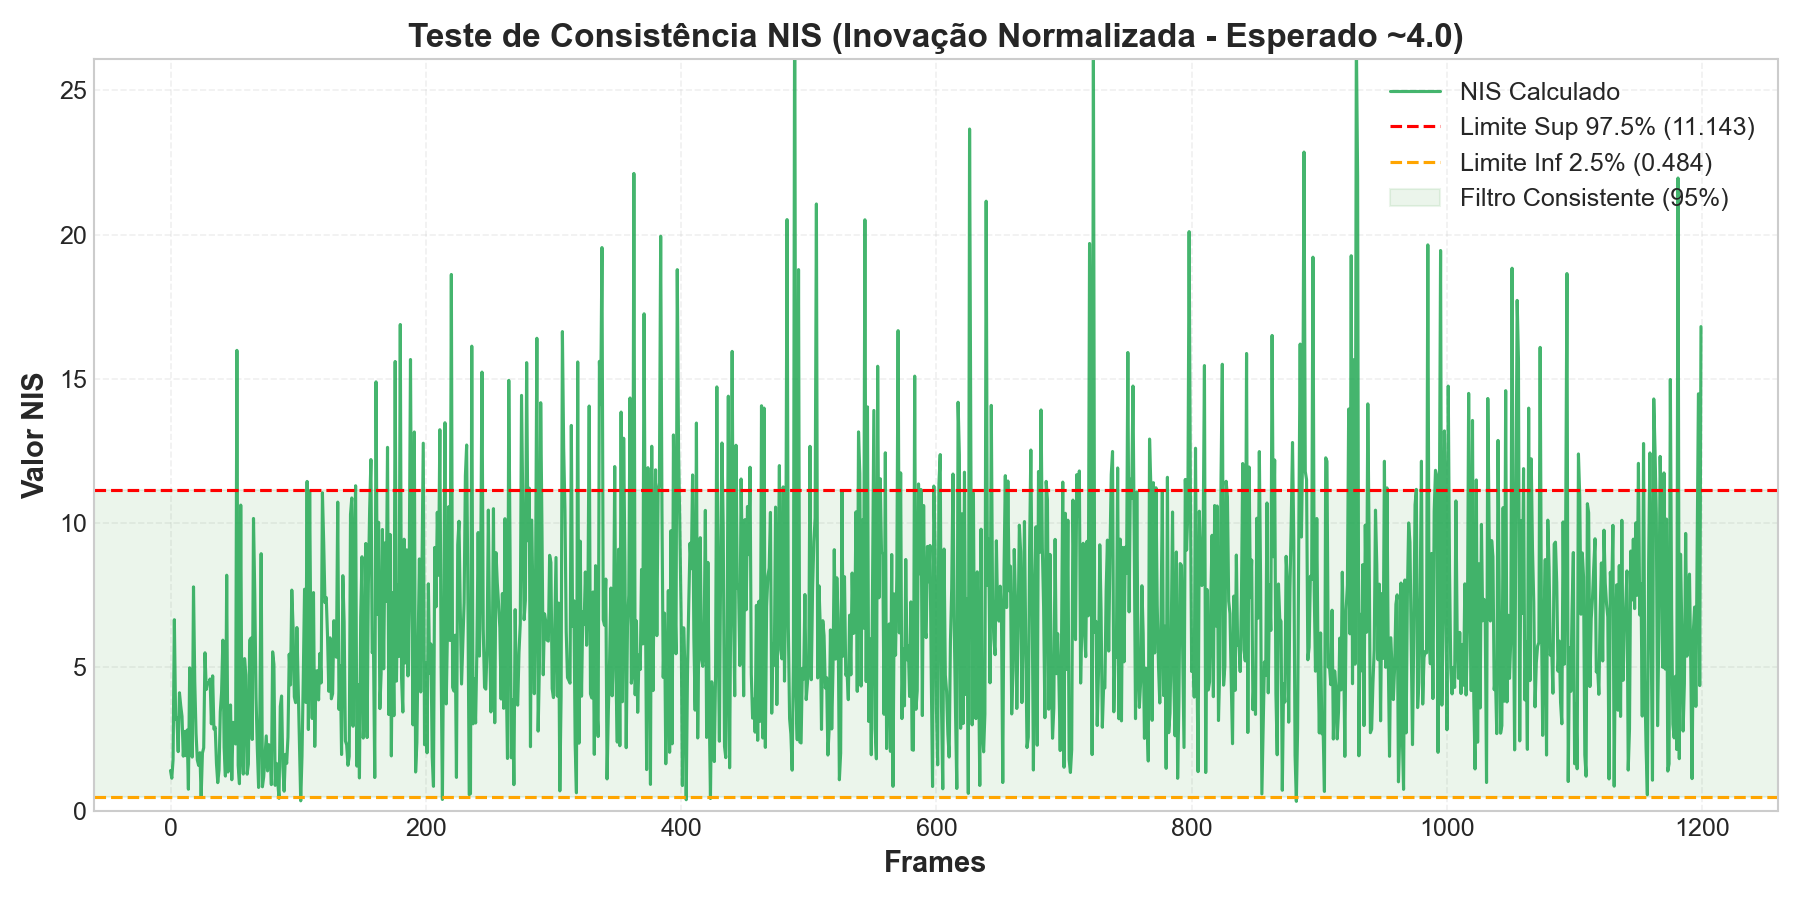
\includegraphics[width=\linewidth]{Figuras/C1/nsintonizado/simulacao_círculo_4_nis.png}
        \vspace{1mm} \par {\small (a) Círculo}
    \end{minipage}
    \hfill
    \begin{minipage}[b]{0.32\linewidth}
        \centering
        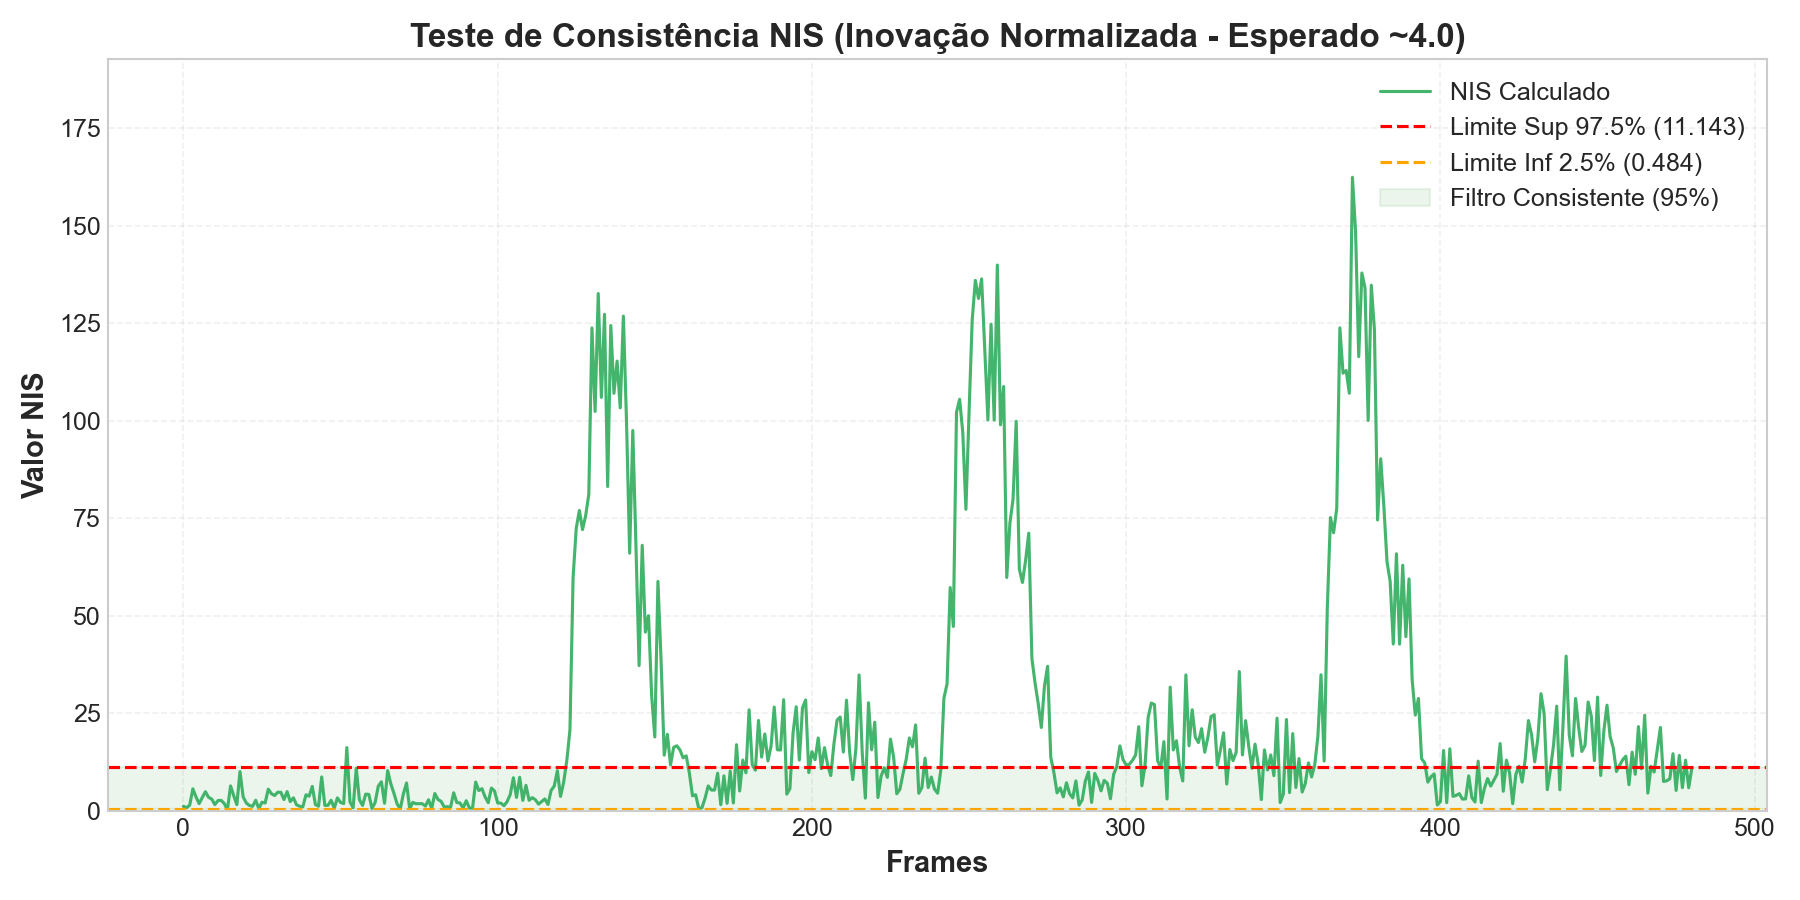
\includegraphics[width=\linewidth]{Figuras/C2/nsintonizado/simulacao_quadrado_4_nis.png}
        \vspace{1mm} \par {\small (b) Quadrado}
    \end{minipage}
    \hfill
    \begin{minipage}[b]{0.32\linewidth}
        \centering
        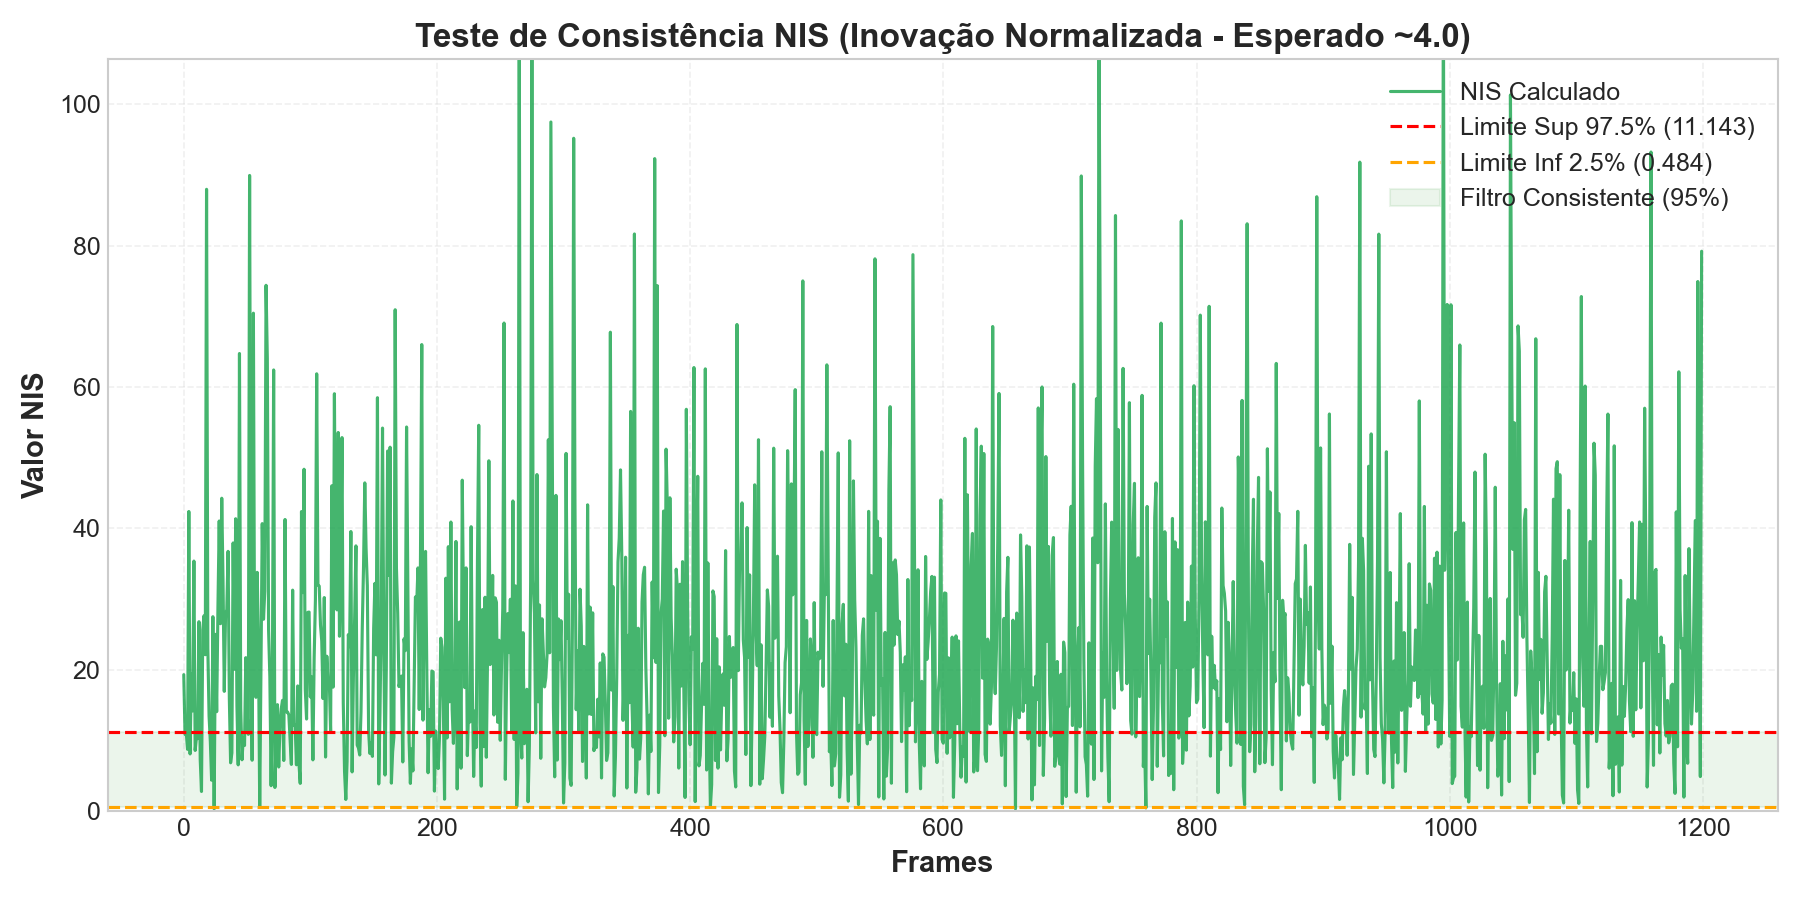
\includegraphics[width=\linewidth]{Figuras/C3/nsintonizado/simulacao_tangente_hiperbólica_4_nis.png}
        \vspace{1mm} \par {\small (c) Tangente Hiperbólica}
    \end{minipage}
    
    \vspace{3mm}
    
    % Linha 2
    \begin{minipage}[b]{0.32\linewidth}
        \centering
        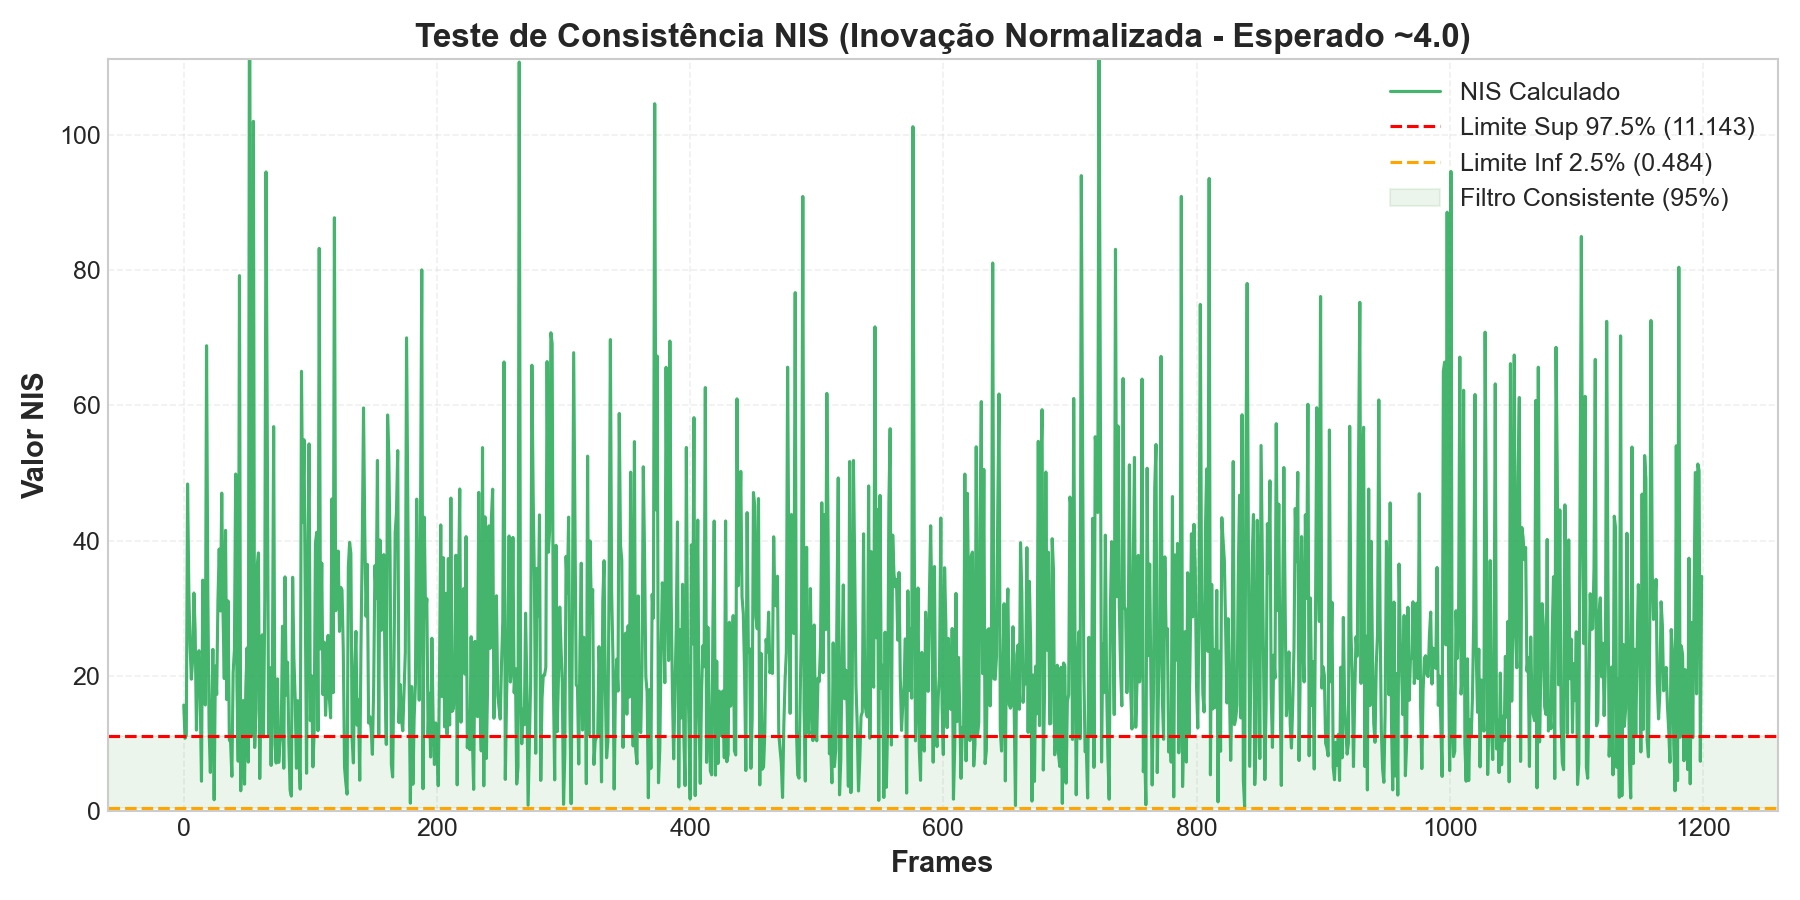
\includegraphics[width=\linewidth]{Figuras/C4/nsintonizado/simulacao_lemniscata_4_nis.png}
        \vspace{1mm} \par {\small (d) Lemniscata}
    \end{minipage}
    \hfill
    \begin{minipage}[b]{0.32\linewidth}
        \centering
        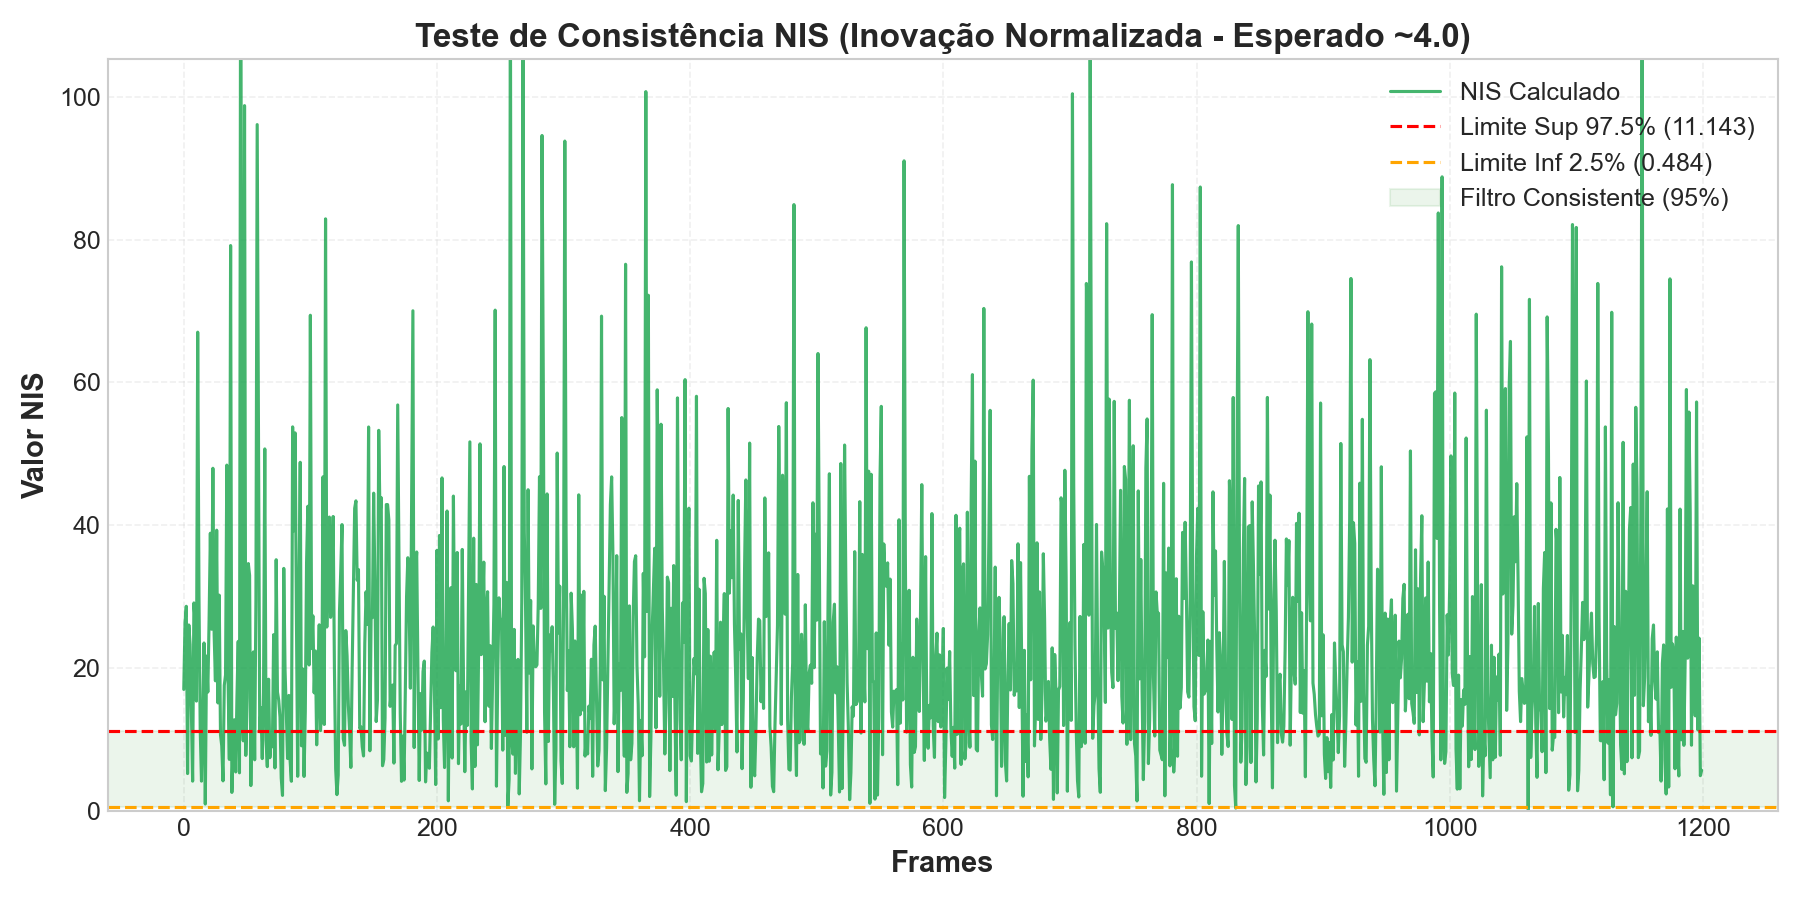
\includegraphics[width=\linewidth]{Figuras/C5/nsintonizado/simulacao_aleatória_4_nis.png}
        \vspace{1mm} \par {\small (e) Aleatória}
    \end{minipage}
    \hfill
    \begin{minipage}[b]{0.32\linewidth}
        \centering
        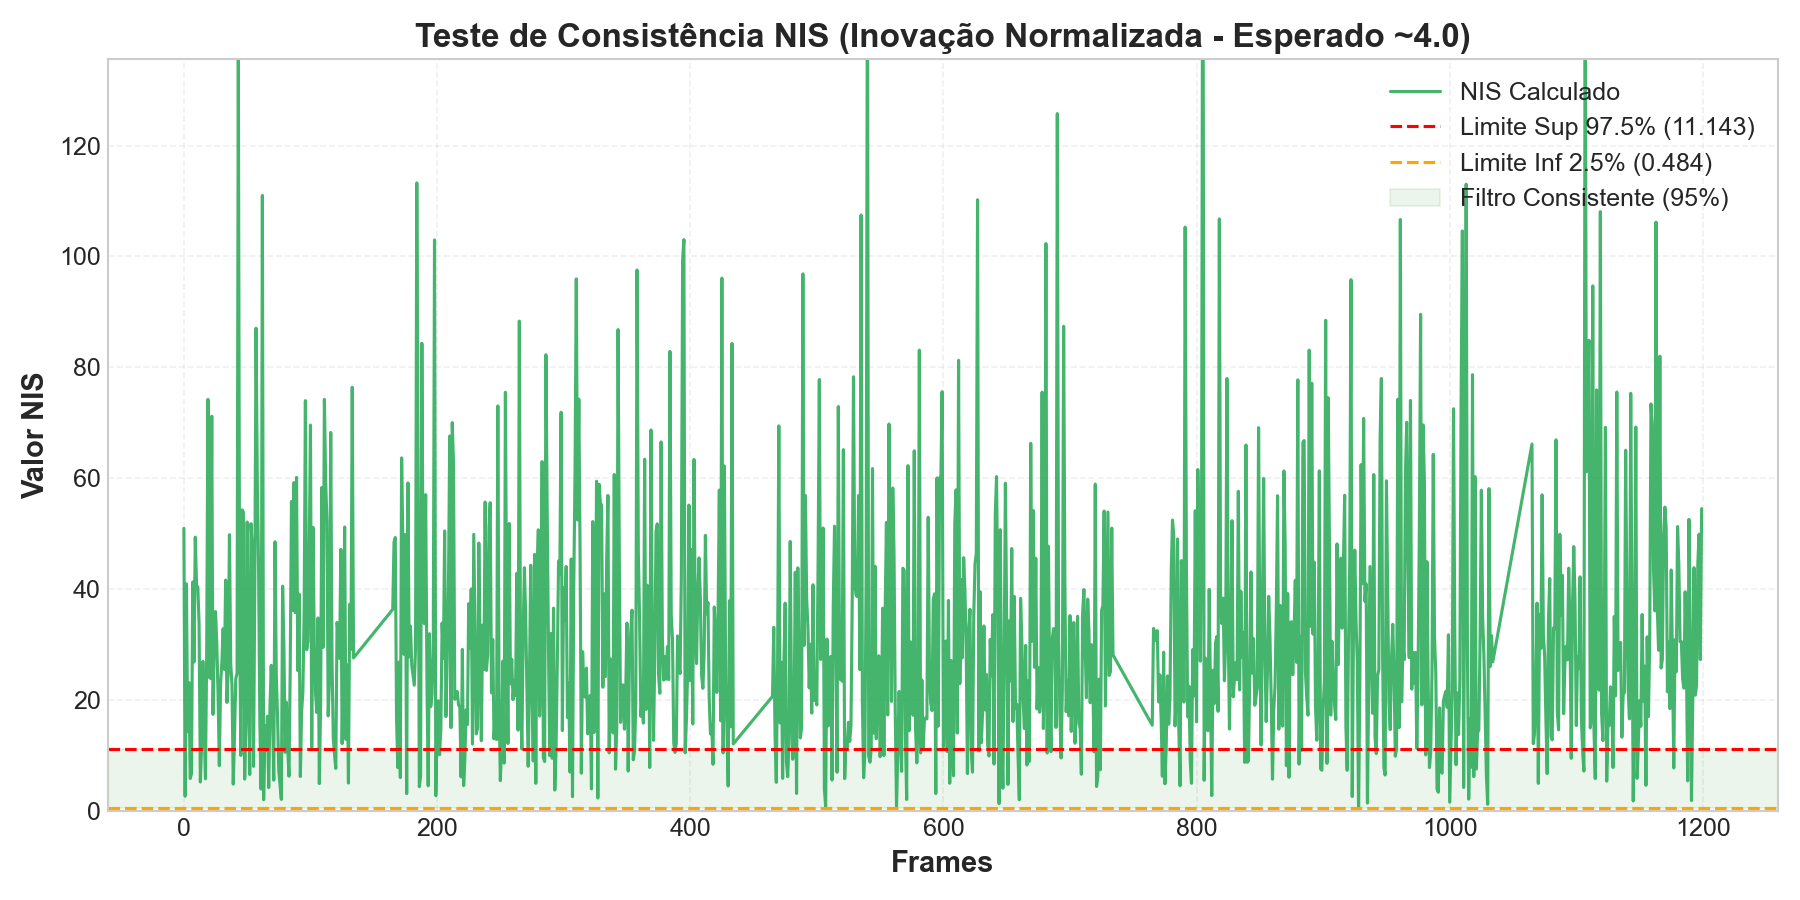
\includegraphics[width=\linewidth]{Figuras/C6/nsintonizado/simulacao_oclusão_4_nis.png}
        \vspace{1mm} \par {\small (f) Oclusão}
    \end{minipage}
    
    \caption{Evolução temporal da métrica NIS para a \textbf{condição não sintonizada}. A constante violação do limiar estatístico evidencia a degradação estrutural e a perda de confiança na matriz de covariância preditiva.}
    \label{fig:app_nis_naosintonizado_grid}
\end{figure*}

% QUEBRA DE PÁGINA OBRIGATÓRIA
\clearpage

% ==============================================================
% PÁGINA 4: TODOS OS GRÁFICOS HISTOGRAMAS (SINTONIZADOS E NÃO SINTONIZADOS) - MAIORES
% ==============================================================
\begin{figure*}[!htpb]
    \centering
    
    % --- PARTE A: HISTOGRAMA SINTONIZADO ---
    % Linha 1
    \begin{minipage}[b]{0.32\linewidth}
        \centering
        
\includegraphics[width=\linewidth]{Figuras/C1/sintonizado/simulacao_círculo_5_hist.png}
        \vspace{1mm} \par {\small (a) Círculo}
    \end{minipage}
    \hfill
    \begin{minipage}[b]{0.32\linewidth}
        \centering
        
\includegraphics[width=\linewidth]{Figuras/C2/sintonizado/simulacao_quadrado_5_hist.png}
        \vspace{1mm} \par {\small (b) Quadrado}
    \end{minipage}
    \hfill
    \begin{minipage}[b]{0.32\linewidth}
        \centering
        
\includegraphics[width=\linewidth]{Figuras/C3/sintonizado/simulacao_tangente_hiperbólica_5_hist.png}
        \vspace{1mm} \par {\small (c) Tangente Hiperbólica}
    \end{minipage}
    
    \vspace{3mm}
    
    % Linha 2
    \begin{minipage}[b]{0.32\linewidth}
        \centering
        
\includegraphics[width=\linewidth]{Figuras/C4/sintonizado/simulacao_lemniscata_5_hist.png}
        \vspace{1mm} \par {\small (d) Lemniscata}
    \end{minipage}
    \hfill
    \begin{minipage}[b]{0.32\linewidth}
        \centering
        
\includegraphics[width=\linewidth]{Figuras/C5/sintonizado/simulacao_aleatória_5_hist.png}
        \vspace{1mm} \par {\small (e) Aleatória}
    \end{minipage}
    \hfill
    \begin{minipage}[b]{0.32\linewidth}
        \centering
        
\includegraphics[width=\linewidth]{Figuras/C6/sintonizado/simulacao_oclusão_5_hist.png}
        \vspace{1mm} \par {\small (f) Oclusão}
    \end{minipage}
    
    \caption{Distribuição dos resíduos (histogramas) para a \textbf{condição sintonizada}. Os perfis mantêm forte aderência à distribuição normal, indicando que as inovações do filtro são não viesadas.}
    \label{fig:app_hist_sintonizado_grid}

    \vspace{8mm} % ESPAÇO ENTRE OS DOIS BLOCOS DE HISTOGRAMAS

    % --- PARTE B: HISTOGRAMA NÃO SINTONIZADO ---
    % Linha 1
    \begin{minipage}[b]{0.32\linewidth}
        \centering
        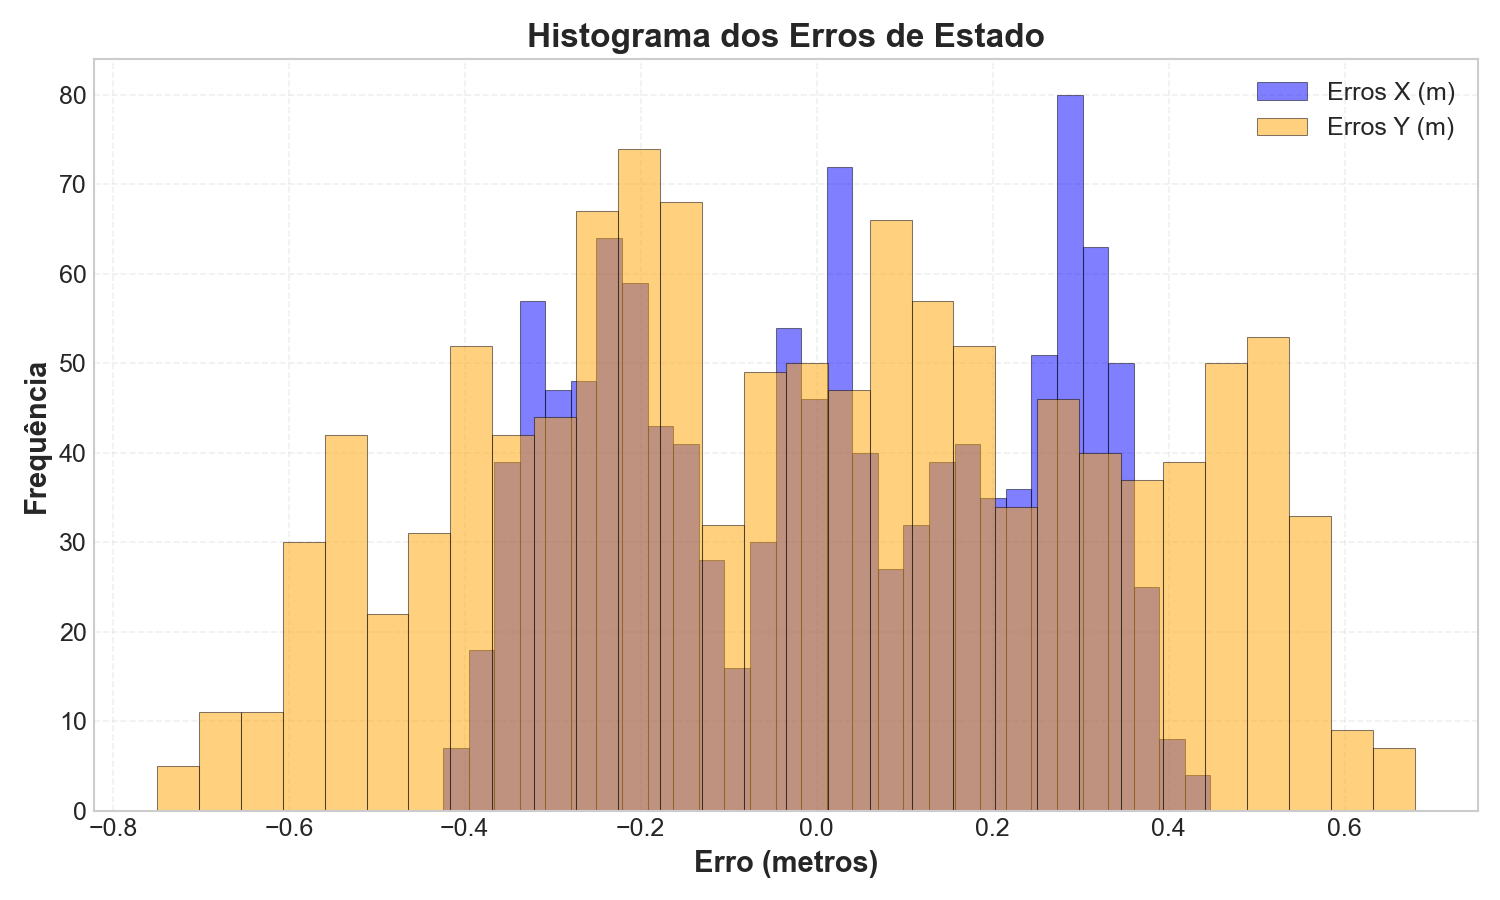
\includegraphics[width=\linewidth]{Figuras/C1/nsintonizado/simulacao_círculo_5_hist.png}
        \vspace{1mm} \par {\small (a) Círculo}
    \end{minipage}
    \hfill
    \begin{minipage}[b]{0.32\linewidth}
        \centering
        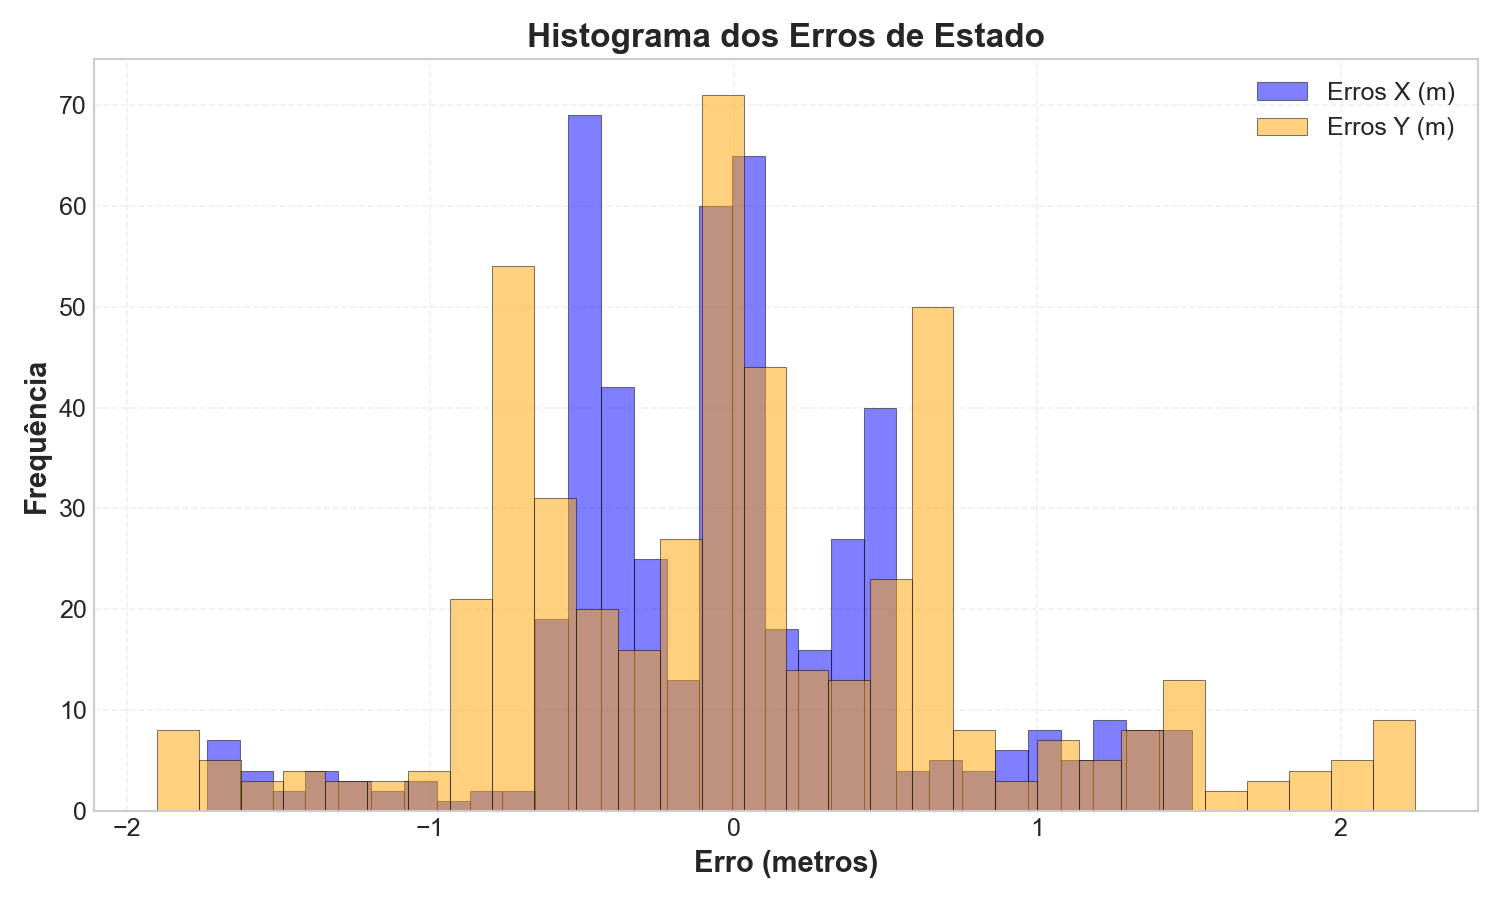
\includegraphics[width=\linewidth]{Figuras/C2/nsintonizado/simulacao_quadrado_5_hist.png}
        \vspace{1mm} \par {\small (b) Quadrado}
    \end{minipage}
    \hfill
    \begin{minipage}[b]{0.32\linewidth}
        \centering
        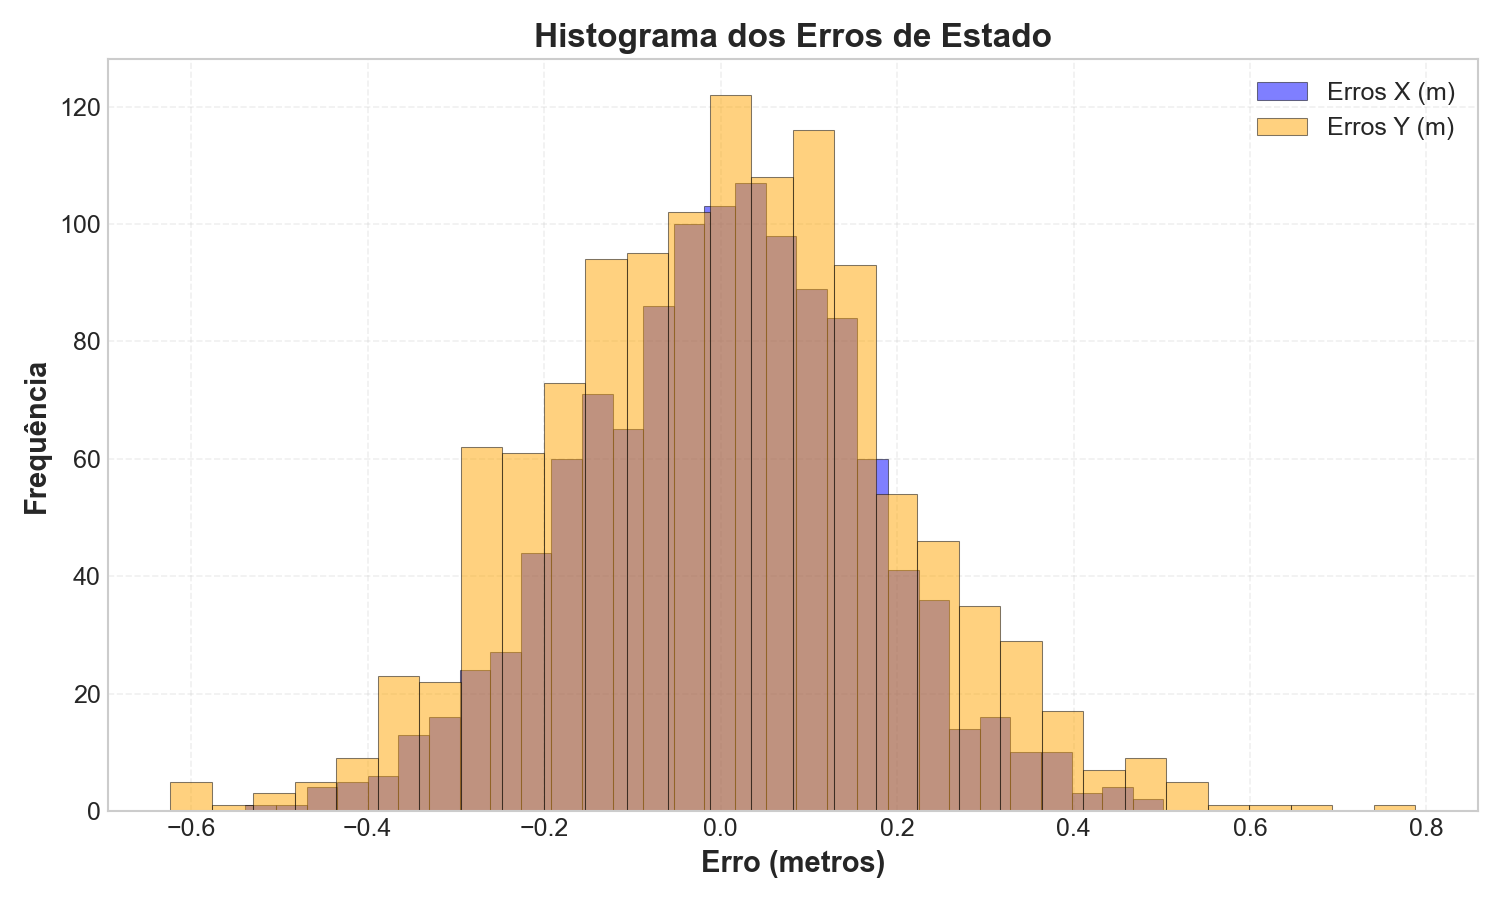
\includegraphics[width=\linewidth]{Figuras/C3/nsintonizado/simulacao_tangente_hiperbólica_5_hist.png}
        \vspace{1mm} \par {\small (c) Tangente Hiperbólica}
    \end{minipage}
    
    \vspace{3mm}
    
    % Linha 2
    \begin{minipage}[b]{0.32\linewidth}
        \centering
        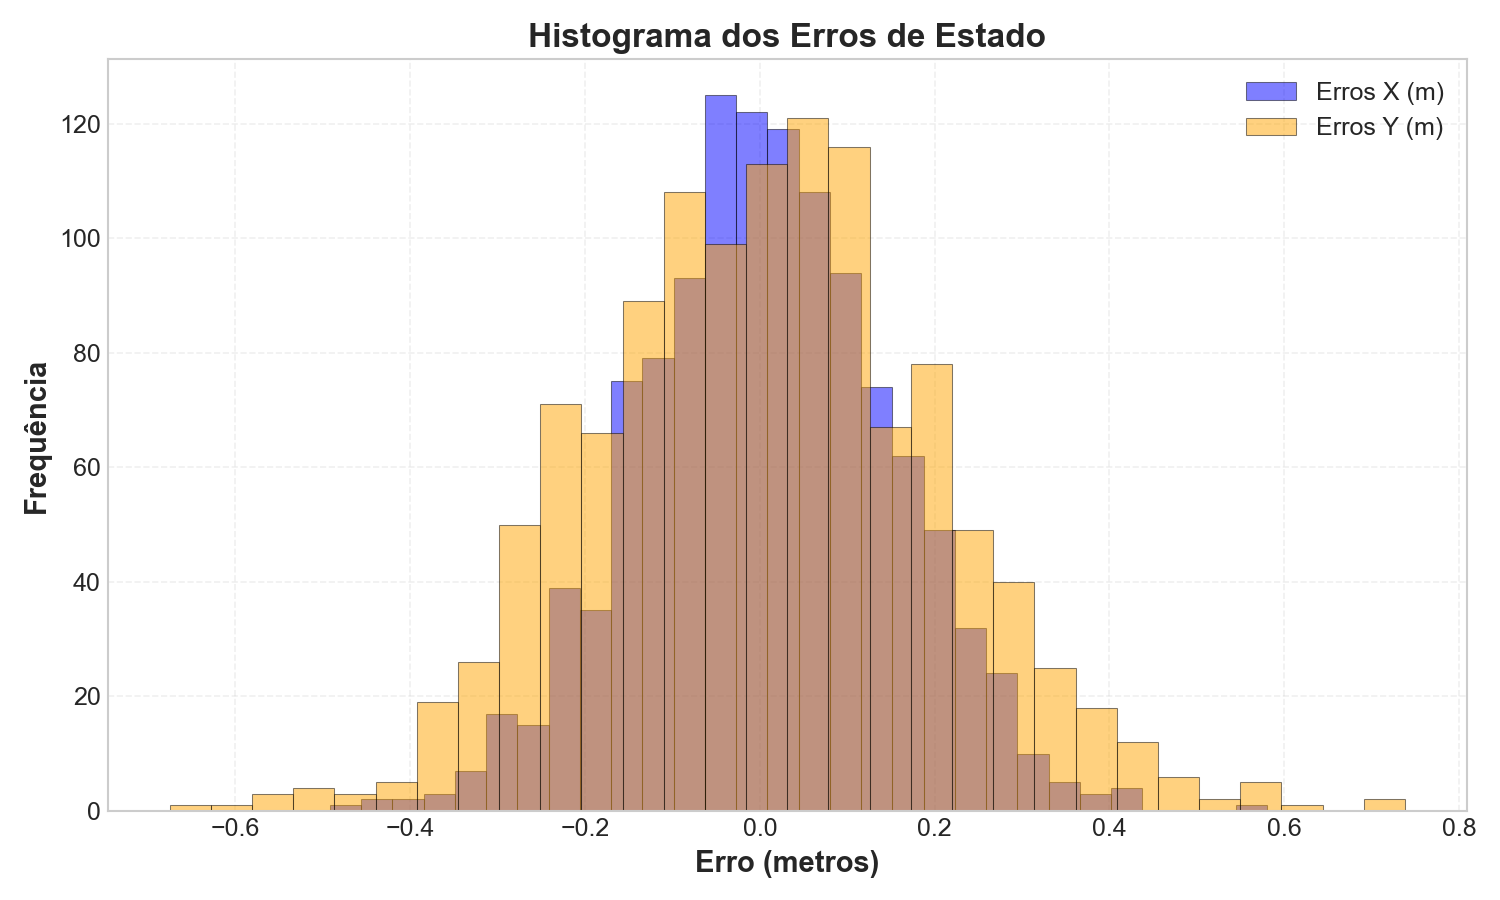
\includegraphics[width=\linewidth]{Figuras/C4/nsintonizado/simulacao_lemniscata_5_hist.png}
        \vspace{1mm} \par {\small (d) Lemniscata}
    \end{minipage}
    \hfill
    \begin{minipage}[b]{0.32\linewidth}
        \centering
        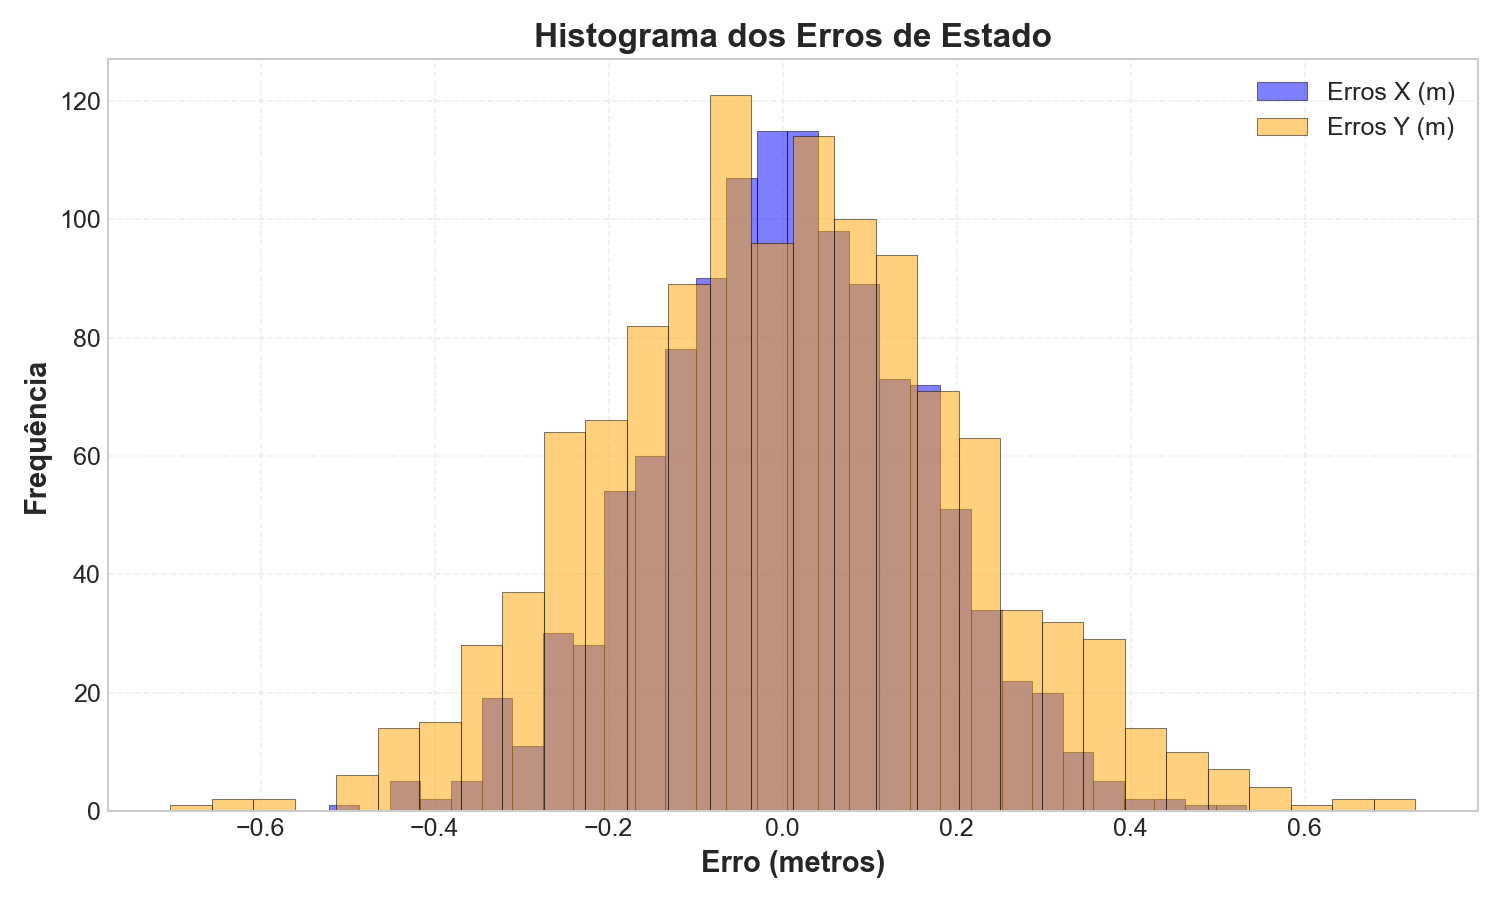
\includegraphics[width=\linewidth]{Figuras/C5/nsintonizado/simulacao_aleatória_5_hist.png}
        \vspace{1mm} \par {\small (e) Aleatória}
    \end{minipage}
    \hfill
    \begin{minipage}[b]{0.32\linewidth}
        \centering
        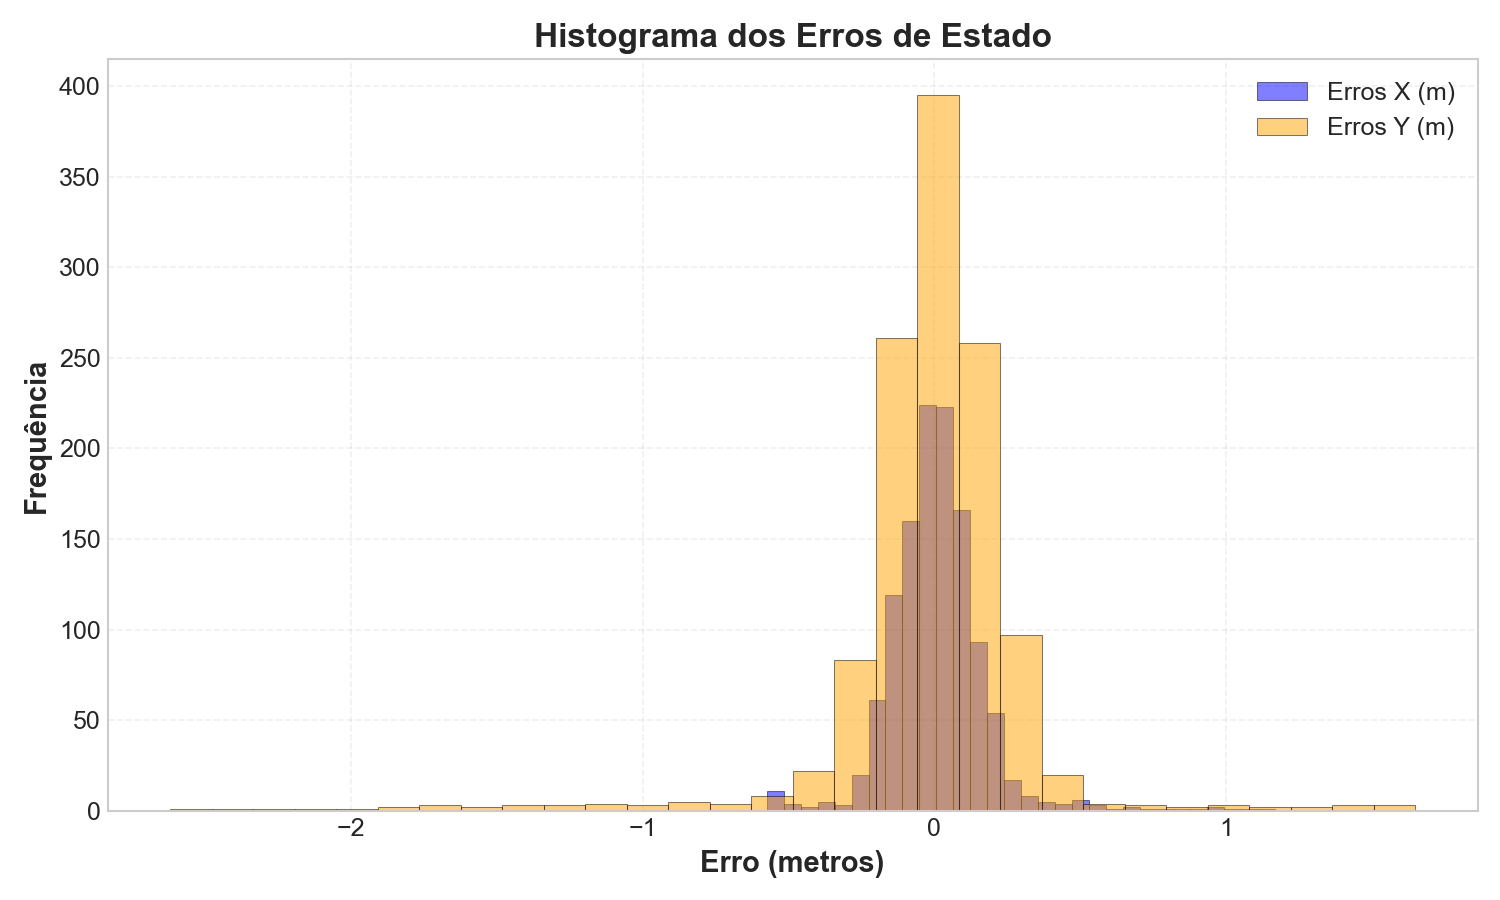
\includegraphics[width=\linewidth]{Figuras/C6/nsintonizado/simulacao_oclusão_5_hist.png}
        \vspace{1mm} \par {\small (f) Oclusão}
    \end{minipage}

    \caption{Distribuição dos resíduos (histogramas) para a \textbf{condição não sintonizada}. Observa-se a acentuada perda de normalidade e o surgimento de assimetrias, o que caracteriza um comportamento subótimo.}
    \label{fig:app_hist_naosintonizado_grid}
\end{figure*}

% QUEBRA DE PÁGINA OBRIGATÓRIA
\clearpage

% ==============================================================
% PÁGINA 5: TODOS OS GRÁFICOS SCATTER (SINTONIZADOS E NÃO SINTONIZADOS) - MAIORES
% ==============================================================
\begin{figure*}[!htpb]
    \centering
    
    % --- PARTE A: SCATTER SINTONIZADO ---
    % Linha 1
    \begin{minipage}[b]{0.24\linewidth}
        \centering
        
\includegraphics[width=\linewidth]{Figuras/C1/sintonizado/simulacao_círculo_3_scatter.png}
        \vspace{1mm} \par {\small (a) Círculo}
    \end{minipage}
    \hfill
    \begin{minipage}[b]{0.24\linewidth}
        \centering
        
\includegraphics[width=\linewidth]{Figuras/C2/sintonizado/simulacao_quadrado_3_scatter.png}
        \vspace{1mm} \par {\small (b) Quadrado}
    \end{minipage}
    \hfill
    \begin{minipage}[b]{0.24\linewidth}
        \centering
        
\includegraphics[width=\linewidth]{Figuras/C3/sintonizado/simulacao_tangente_hiperbólica_3_scatter.png}
        \vspace{1mm} \par {\small (c) Tangente Hiperbólica}
    \end{minipage}
    
    \vspace{3mm}
    
    % Linha 2
    \begin{minipage}[b]{0.24\linewidth}
        \centering
        
\includegraphics[width=\linewidth]{Figuras/C4/sintonizado/simulacao_lemniscata_3_scatter.png}
        \vspace{1mm} \par {\small (d) Lemniscata}
    \end{minipage}
    \hfill
    \begin{minipage}[b]{0.24\linewidth}
        \centering
        
\includegraphics[width=\linewidth]{Figuras/C5/sintonizado/simulacao_aleatória_3_scatter.png}
        \vspace{1mm} \par {\small (e) Aleatória}
    \end{minipage}
    \hfill
    \begin{minipage}[b]{0.24\linewidth}
        \centering
        
\includegraphics[width=\linewidth]{Figuras/C6/sintonizado/simulacao_oclusão_3_scatter.png}
        \vspace{1mm} \par {\small (f) Oclusão}
    \end{minipage}
    
    \caption{Gráficos de dispersão (\textit{scatter plots}) das inovações para a \textbf{condição sintonizada}. Os pontos concentram-se simetricamente em torno da origem, refletindo a eficácia do estimador na modelagem do ruído.}
    \label{fig:app_scatter_sintonizado_grid}

    \vspace{8mm} % ESPAÇO ENTRE OS DOIS BLOCOS DE SCATTER

    % --- PARTE B: SCATTER NÃO SINTONIZADO ---
    % Linha 1
    \begin{minipage}[b]{0.24\linewidth}
        \centering
        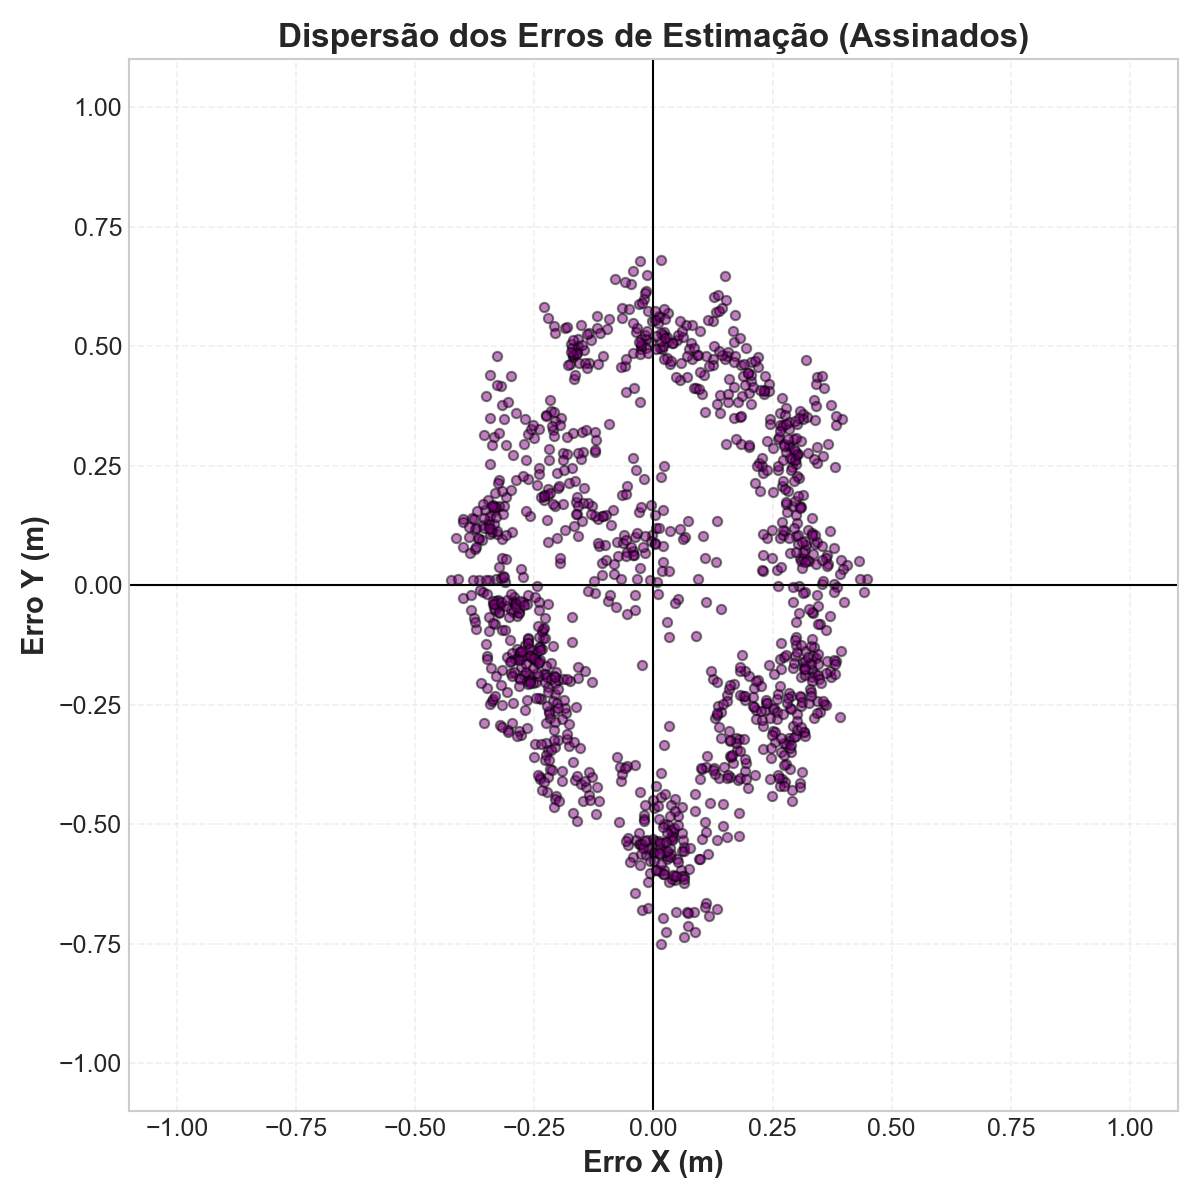
\includegraphics[width=\linewidth]{Figuras/C1/nsintonizado/simulacao_círculo_3_scatter.png}
        \vspace{1mm} \par {\small (a) Círculo}
    \end{minipage}
    \hfill
    \begin{minipage}[b]{0.24\linewidth}
        \centering
        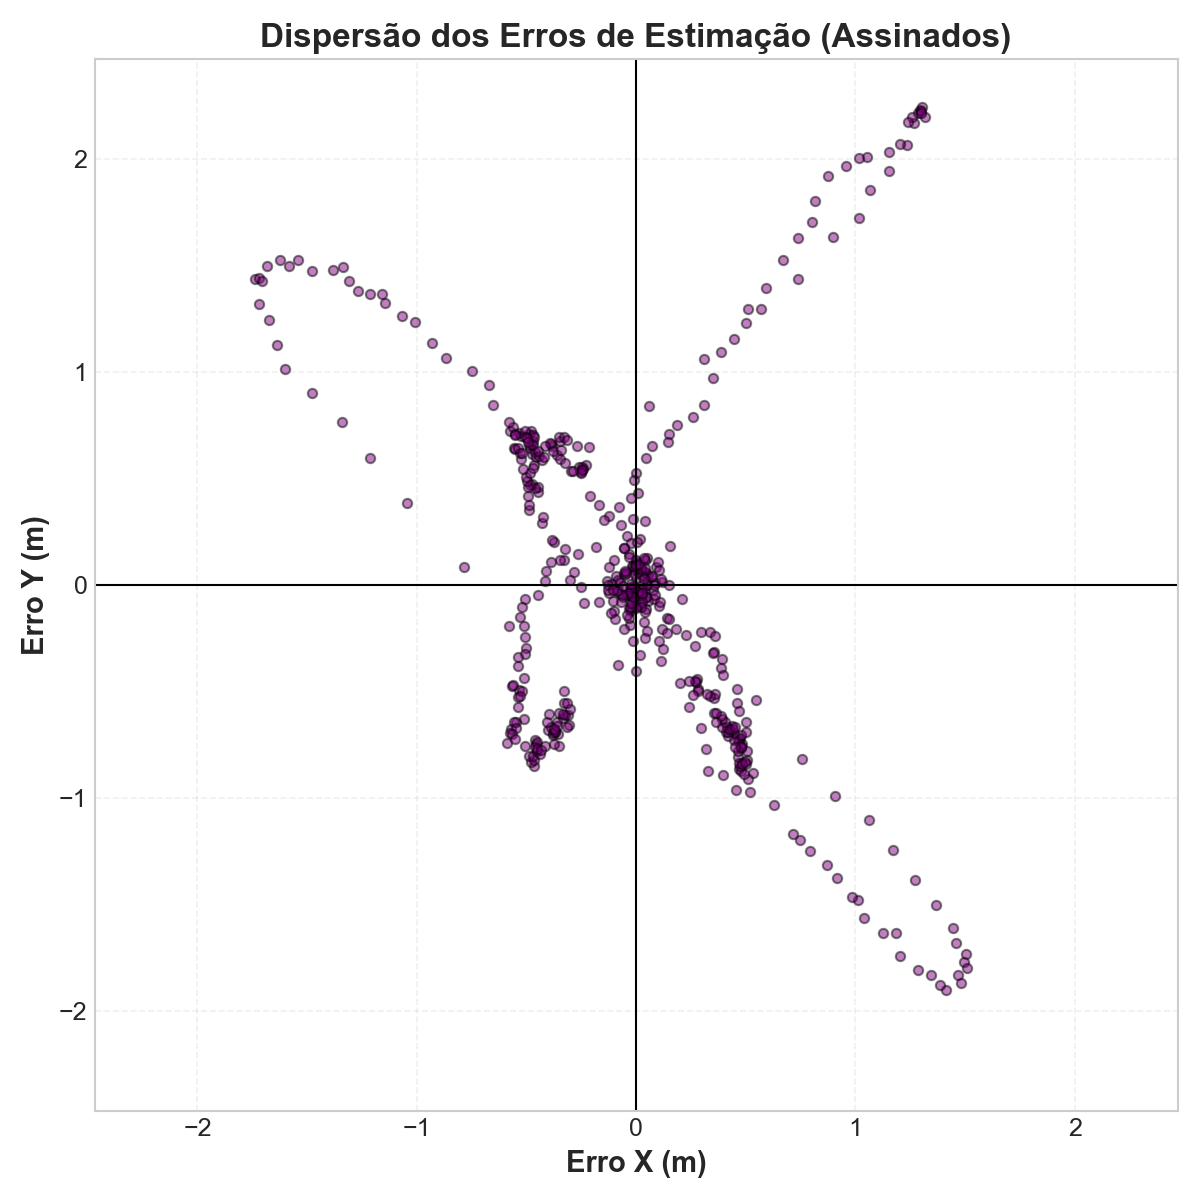
\includegraphics[width=\linewidth]{Figuras/C2/nsintonizado/simulacao_quadrado_3_scatter.png}
        \vspace{1mm} \par {\small (b) Quadrado}
    \end{minipage}
    \hfill
    \begin{minipage}[b]{0.24\linewidth}
        \centering
        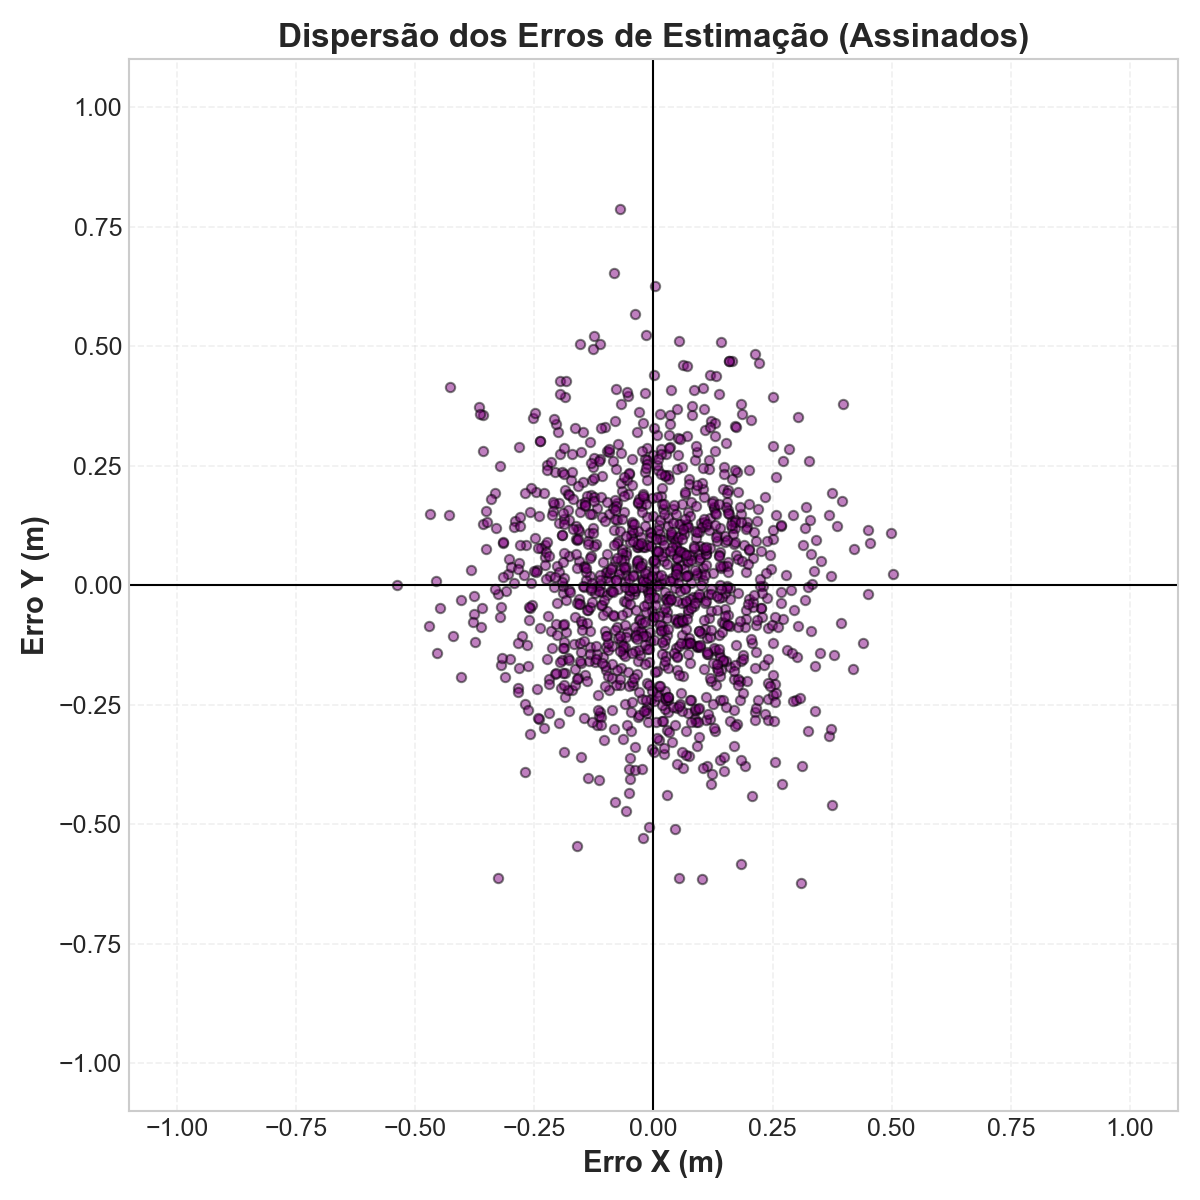
\includegraphics[width=\linewidth]{Figuras/C3/nsintonizado/simulacao_tangente_hiperbólica_3_scatter.png}
        \vspace{1mm} \par {\small (c) Tangente Hiperbólica}
    \end{minipage}
    
    \vspace{3mm}
    
    % Linha 2
    \begin{minipage}[b]{0.24\linewidth}
        \centering
        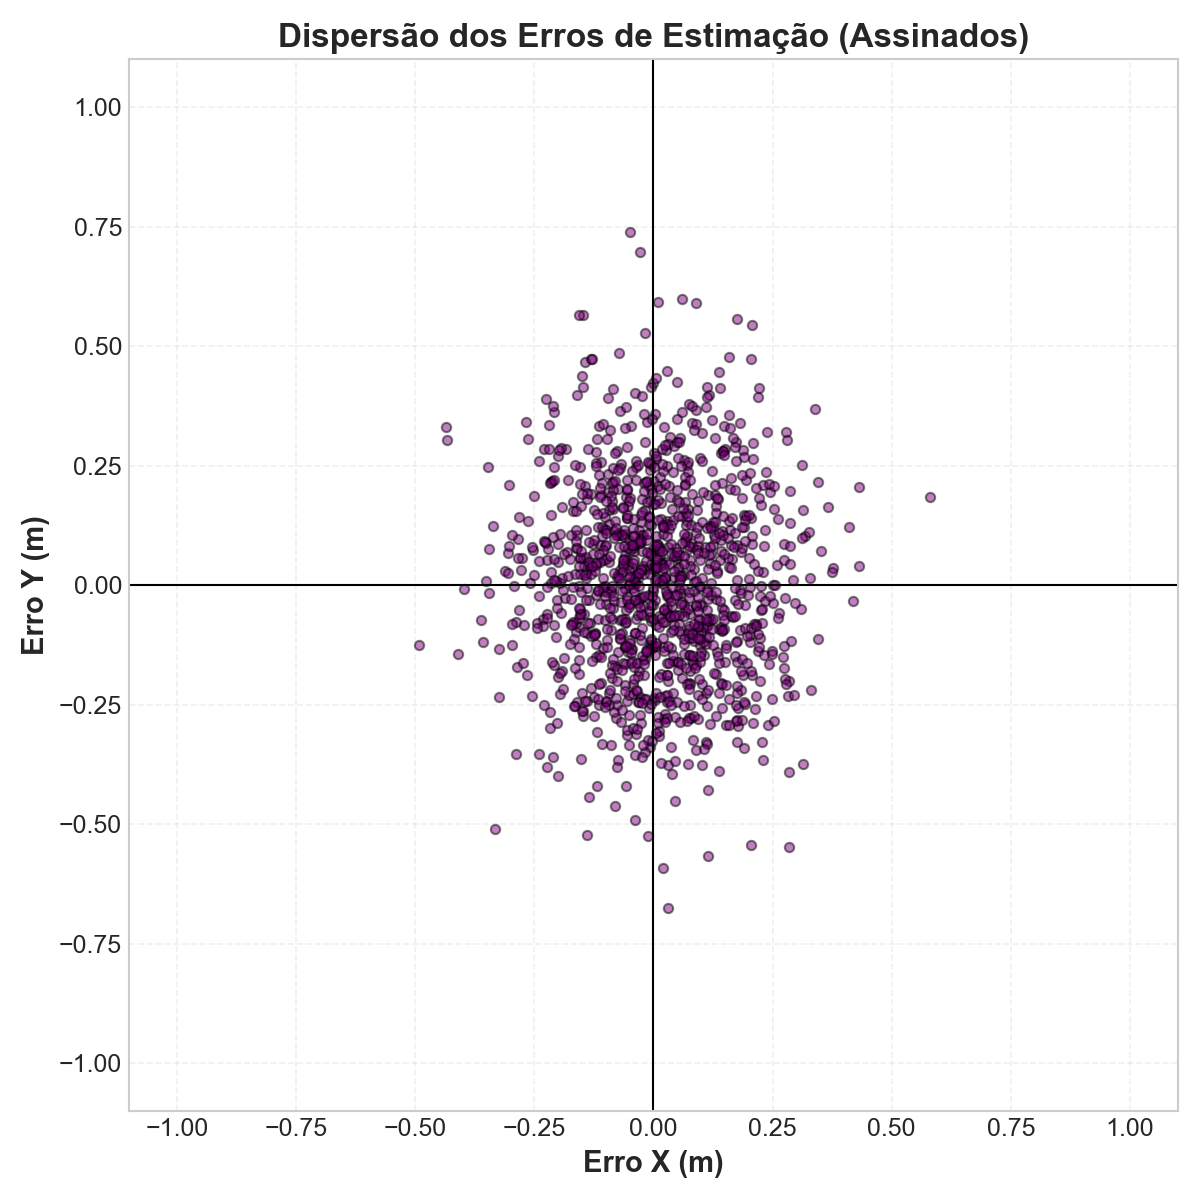
\includegraphics[width=\linewidth]{Figuras/C4/nsintonizado/simulacao_lemniscata_3_scatter.png}
        \vspace{1mm} \par {\small (d) Lemniscata}
    \end{minipage}
    \hfill
    \begin{minipage}[b]{0.24\linewidth}
        \centering
        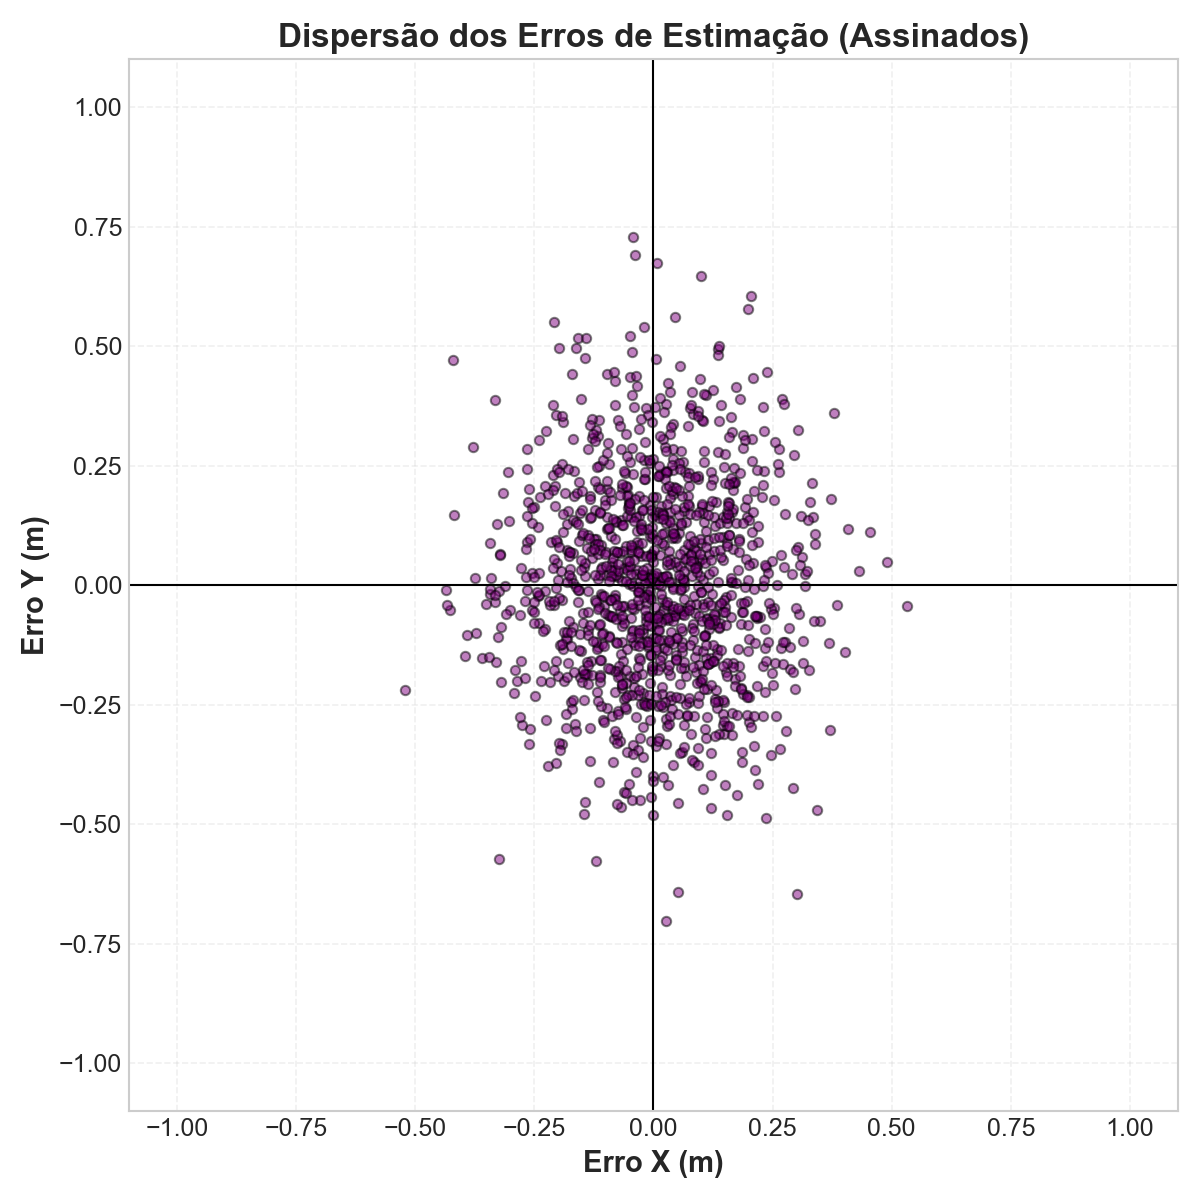
\includegraphics[width=\linewidth]{Figuras/C5/nsintonizado/simulacao_aleatória_3_scatter.png}
        \vspace{1mm} \par {\small (e) Aleatória}
    \end{minipage}
    \hfill
    \begin{minipage}[b]{0.24\linewidth}
        \centering
        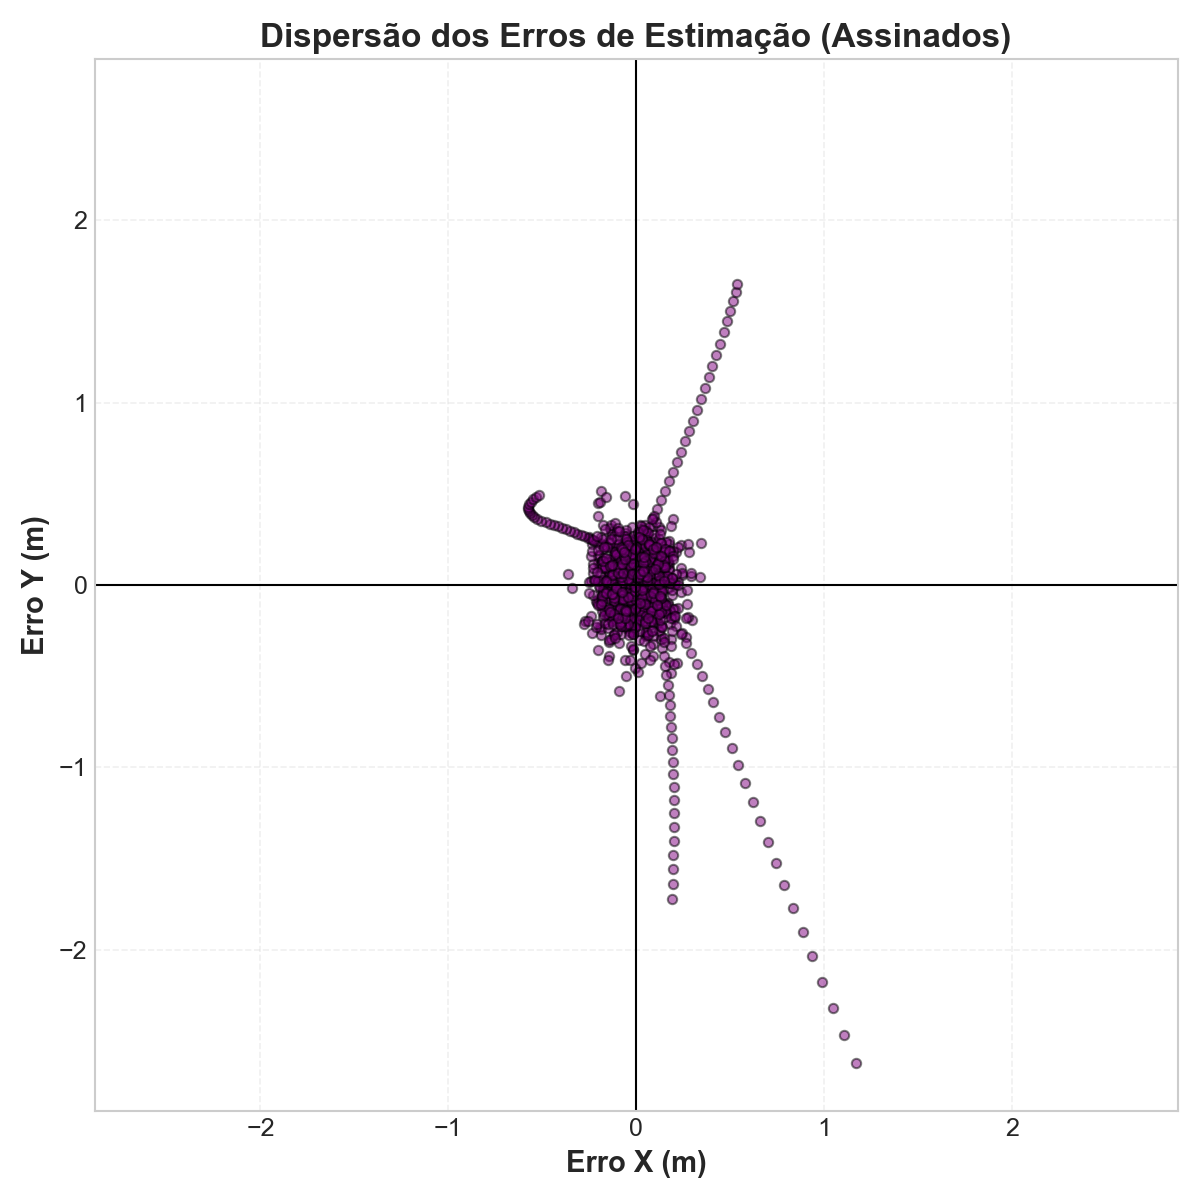
\includegraphics[width=\linewidth]{Figuras/C6/nsintonizado/simulacao_oclusão_3_scatter.png}
        \vspace{1mm} \par {\small (f) Oclusão}
    \end{minipage}

    \caption{Gráficos de dispersão das inovações para a \textbf{condição não sintonizada}. A dispersão irregular e o distanciamento acentuado da origem denotam a introdução de viés e a imprecisão preditiva do modelo.}
    \label{fig:app_scatter_naosintonizado_grid}
\end{figure*}